\documentclass[letterpaper, 12pt, oneside]{tesis}

% Paquetes para idioma
\usepackage[spanish]{babel}
\usepackage[utf8]{inputenc}
\usepackage[fixlanguage]{babelbib}

% Otros paquetes instalados
% Básicos
\usepackage{natbib}
\usepackage{enumerate}

% Para dibujar figuras
\usepackage{tikz}

% Para cambiar el color de las letras
\usepackage{color}

% Para incluir código (básico)
\usepackage{verbatim}
\usepackage{fancyvrb}

% Para incluir hipervínculos
\usepackage{hyperref}
\hypersetup{urlcolor=blue, colorlinks=false}

% Para más símbolos matemáticos
\usepackage{amsmath}
\usepackage{amsthm}
\usepackage{amssymb}

% Para colocar teoremas en cajas
\usepackage{mdframed}

% Para texto Lorem Ipsum
\usepackage{blindtext}

% Paquetes locales
% Puedes agregar paquetes locales (archivos .sty) en un subdirectorio % 'paquetes'.
% Utiliza la sintaxis \usepackage{paquetes/nombrePaquete}

% Todas las imágenes se cargan del subdirectorio 'img' por defecto.
\graphicspath{{img/}}

% Sangrías de 3 espacios (3 veces el espacio de la x)
\parindent 3ex 

% Interlineado
\setlength{\baselineskip}{1.5pt}

% Interpárrafo
\setlength{\parskip}{16.5pt}

\topmargin 2cm

\renewcommand{\tablename}{Tabla}
\newcommand\listsymbolname{Acrónimos y Símbolos}

\begin{titlepage}
    \title{\vspace{-2cm} 
\includegraphics[width=1.2in]{./usb.png} \\[.2cm]
        \large Universidad Simón Bolívar \\
        Decanato de Estudios Profesionales \\
        Coordinación de Ingeniería de la Computación
        \vfill \LARGE @títuloProyecto \vfill}
    \author{Por: \\
        @autor1 \\
        @autor2 \\[1.2cm]
        Realizado con la asesoría de: \\
        @tutor \\[1.2cm]
        PROYECTO DE GRADO \\
Presentado ante la Ilustre Universidad Simón Bolívar \\
como requisito parcial para optar al título de \\
Ingeniero de Computación}
    \date{Sartenejas, @mes de @año}
\end{titlepage}

\begin{document}
\frontmatter
\maketitle
\setstretch{1.3}

% Se incluye el acta de evaluación, verificar que se corresponda
% con el formato aceptado actualmente por el Decanato.
% Pagina del acta final
\begin{titlepage}
\begin{center}

% Upper part

\includegraphics[scale=0.5]{usb.png} \\

\textsc {\large UNIVERSIDAD SIMÓN BOLÍVAR} \\
\textsc{DECANATO DE ESTUDIOS PROFESIONALES\\
COORDINACIÓN DE INGENIERÍA DE LA COMPUTACIÓN}

\bigskip
\bigskip
\bigskip
\bigskip
\bigskip
\bigskip

% Title
\textsc{ACTA FINAL PROYECTO DE GRADO}

\bigskip
\bigskip

\textsc{\bfseries @títuloProyecto}

\bigskip
\bigskip
\bigskip
\bigskip

\begin{minipage}{\textwidth}
\centering
Presentado por: \\
\textsc{\bfseries @autor1} \\
\textsc{\bfseries @autor2} \\

\bigskip
\bigskip
\bigskip

Este Proyecto de Grado ha sido aprobado por el siguiente jurado examinador: \\

\bigskip
\bigskip

% Despues de cada line coloca el (los) nombre(s) de
% cada uno de los integrantes del jurado.
\line(1,0){200} \\
@tutor\\

\bigskip
\bigskip

\line(1,0){200} \\
@jurado1\\

\bigskip
\bigskip

\line(1,0){200} \\
@jurado2\\
\end{minipage}

\bigskip
\bigskip
\vfill

% Date/Fecha
{\large \bfseries Sartenejas, @día de @mes de @año}

\end{center}
\end{titlepage}
 

% El resumen debe ser de una sola página
\addtotoc{Resumen}
\abstract{
\addtocontents{toc}{\vspace{1em}}
\blindtext

\blindtext

% Las palabras clave son generalmente los nombres de áreas de investigación a
% los cuales está asociado el trabajo. Generalmente son tres o cuatro.
\noindent \begin{small} \textbf{Palabras clave}: @palabra1, @palabra2, @palabra3.
\end{small}

% Iniciar nueva página luego del resumen
\clearpage
\setstretch{1.3}

% Agradecimientos
\acknowledgements{
\addtocontents{toc}{\vspace{1em}}
\blindtext

\blindtext
}
\clearpage

\pagestyle{fancy}

% Tabla de contenidos o índice
\lhead{\emph{Índice General}}
\tableofcontents

% Estos índices solamente se usan si el libro contiene figuras, tablas y
% algoritmos. Si alguno de estos no se utiliza, comentar o eliminar las líneas
% pertinentes.
\lhead{\emph{Índice de Figuras}}
\listoffigures

\lhead{\emph{Índice de Tablas}}
\renewcommand*\listtablename{Índice de Tablas}
\listoftables

%\lhead{\emph{Índice de Algoritmos}}
%\renewcommand*\listalgorithmname{Índice de algoritmos}
%\listofalgorithms

\setstretch{1.5}
\clearpage
\lhead{\emph{Acrónimos y símbolos}}
\listofsymbols{ll}
{

    % Aquí van las siglas
    \textbf{SIGLAS} & \textbf{S}iglas \textbf{I}sla \textbf{G}rafo 
                      \textbf{L}aos \textbf{A}ve \textbf{S}erpiente\\
    \textbf{ACM} & \textbf{A}ssociation for \textbf{C}omputing \textbf{M}achinery\\
    &\\
    \hline
    &\\

    % Aquí van los símbolos
    $\iff$ & doble implicación, si y sólo si\\
    $\Rightarrow$ & implicación lógica\\
    $[u:=v]$ & sustitución textual de $u$ por $v$
}

%% ----------------------------------------------------------------
% End of the pre-able, contents and lists of things
% Begin the Dedication page

\setstretch{1.3}  % Return the line spacing back to 1.3

\pagestyle{empty}  % Page style needs to be empty for this page

\dedicatory{
    \textbf{Dedicatoria} \bigskip

    A @personasImportantes, por @razonesDedicatoria.
}

\addtocontents{toc}{\vspace{2em}}

\mainmatter
\pagestyle{fancy}

% Se incluye el cuerpo de la tesis en este documento.

\chapter*{Introducción}
\label{intro}
\setchapter{\emph{Introducción}}

Históricamente, y por varios años, en los cursos de Laboratorio de Algoritmos I
y II dictados en la Universidad Simón Bolívar, el lenguaje de programación
utilizado para la instrucción fue GaCeLa, basado en el lenguaje GCL de Edsger
Dijkstra y desarrollado, junto con su compilador, dentro de la Universidad. Este
compilador no generaba código nativo para la plataforma destino, sino que
transformaba el programa a compilar en otro programa escrito en el lenguaje
Java, idealmente con la misma semántica del original. Este programa generado
debía ser ejecutado usando la máquina virtual de Java (JVM o \textit{Java
Virtual Machine} en inglés).

Desafortunadamente, dependiendo del programa en GaCeLa compilado, el programa
generado en Java presentaba errores que no eran reportados sino hasta que se
intentaba ejecutarlo dentro de la JVM, forzando a los estudiantes a modificar
manualmente este archivo generado mecánicamente a fin de poder ejecutarlo,
actividad para la cual claramente no estaban preparados, ni era objeto de
evaluación de los cursos en cuestión. Adicionalmente, no se contaba con el
personal suficiente para mantener el compilador y reparar este tipo de errores a
nivel del compilador en lugar de en el código generado, por lo cual los
profesores que dictaban estas materias cambiaron el lenguaje de instrucción por
otros lenguajes, entre ellos Pascal, Modula 2, JML y Python, cayendo en desuso
al rededor del año 2010. Actualmente, la documentación disponible para GaCeLa es
muy limitada.

En los cursos teóricos de Algoritmos I y II de la Universidad Simón Bolívar, por
otro lado, el lenguaje de instrucción sigue siendo GCL. En consecuencia, los
estudiantes de estos cursos teóricos, que deben ser inscritos simultáneamente
con el laboratorio correspondiente, se ven forzados a hacer una traducción
mental entre los conceptos estudiados en la teoría y los ejercicios elaborados
en el laboratorio.

Durante el año 2015, Joel Araujo y José Luis Jiménez desarrollaron, como
Proyecto de Grado, un nuevo lenguaje, Graciela, y su respectivo compilador. Este
lenguaje cuenta con los tipos básicos \ingra{int}, \ingra{char}, \ingra{float} y
\ingra{boolean}, y arreglos de estos, ofrece instrucciones de lectura,
escritura, asignación, selección y repetición, permite insertar aserciones entre
las instrucciones (posiblemente haciendo uso de cuantificaciones) y permite la
definición de funciones y procedimientos (con los modos \textit{in},
\textit{in-out}, \textit{out} y \textit{ref} para el pase de parámetros). El
compilador desarrollado por Araujo y Jiménez genera código intermedio LLVM que
posteriormente es convertido en código nativo para la plataforma deseada
haciendo uso del \textit{Back-End} de LLVM.

El lenguaje de Araujo y Jiménez tiene todas las características necesarias para
el primer curso práctico de Algoritmos, pero, como lo indican en las
recomendaciones de su Proyecto de Grado, es necesario extender el lenguaje y el
compilador para lograr que estos sean útiles para el segundo curso práctico de
Algoritmos. Específicamente, recomiendan agregar al lenguaje el tipo
\textit{apuntador} y las instrucciones necesarias para manipularlos, y la
posibilidad de crear tipos de dato estructurados con comportamientos definidos
a través de aserciones invariantes.

Así, es evidente la necesidad de agregar estas extensiones al lenguaje Graciela
y a su compilador, dado que son cruciales para el segundo curso práctico de
Algoritmos, concernido precisamente con el manejo de apuntadores y la definición
de tipos estructurados con comportamientos abstractos. Estas extensiones estarán
siempre guiadas por la especificación del lenguaje GCL siempre que esto sea
posible, para continuar la promoción del aprendizaje de la programación usando
métodos formales en apoyo con los cursos teóricos dictados usando el lenguaje
GCL.

\section*{Otros antecedentes}

Además de GaCeLa y Graciela, existen otras implementaciones de las ideas del
lenguaje GCL ajenas a la Universidad Simón Bolívar, entre las cuales se
encuentran el módulo para el lenguaje Perl \texttt{Commands::Guarded} y GCL 1.2.
El primero \todo{decir algo sobre commands::guarded}, mientras que el segundo es
un interpretador escrito en Prolog y C que impone muchas restricciones sobre
arreglos y aserciones, y no soporta la declaración de procedimientos y
funciones.

\section*{Objetivo General}

Extender el compilador del lenguaje Graciela, una variante del GCL (Guarded
Command Language) de Dijkstra, implantado por Araujo y Jiménez. Esta extensión
deberá soportar tipos de dato definidos por el programador, apuntadores
explícitos, manejo de memoria automático, y un mecanismo de aserciones
verificables que soporte estas nuevas capacidades.

\section*{Objetivos Específicos}
\begin{itemize}
  \item Revisión bibliográfica relacionada con implantación de compiladores,
  sistemas de tipos y semántica axiomática.

  \item Especificación formal de la extensión a Graciela a implantar.

  \item Evaluación de herramientas que faciliten la construcción del ambiente de
  ejecución final para manejo automático de memoria.

  \item Implantación del compilador de la extensión de Graciela a código de
  máquina nativo.

  \item Extensión del manual de usuario con las nuevas funcionalidades.
\end{itemize}

\section*{Organización del Trabajo}

Este Proyecto de Grado se presenta en cuatro capítulos. En el primero, se
establece un marco teórico al cual se hace referencia en los capítulos
subsiguientes, y que permite establecer un nivel de abstracción apropiado para
estos. En el segundo, similarmente, se establece un marco tecnológico, en el
cual se exponen las herramientas que permitieron desarrollar el proyecto en su
forma actual. En el tercer capítulo, el desarrollo del proyecto, se detalla el
estudio que se realizó de las recomendaciones dadas por Araujo y Jiménez y las
consideraciones que se tomaron en cuenta para cumplir estas recomendaciones y
los objetivos especificados para este proyecto, incluyendo también el proceso de
desarrollo asociado a los objetivos adicionales que surgieron durante el
desarrollo del mismo. En el cuarto capítulo se exponen los resultados del
proyecto, describiendo con detalle la sintaxis definitiva incorporada al
lenguaje Graciela y la explicación de la semántica de estas extensiones, así
como las herramientas y utilidades que se desarrollaron para facilitar el uso de
dicho lenguaje.


% El número de capítulos varía. En mi libro fueron cuatro (sin contar
% introducción y conclusión).
\chapter{Marco Teórico}
\label{capitulo1}
\lhead{Capítulo 1. \emph{Marco Teórico}}

\section{Programación formal y tripletas de Hoare}

\section{Teoría de conjuntos}

La Teoría de Conjuntos es la rama de la matemática que se encarga del estudio de
colecciones bien formados de objetos, que pueden o no ser de naturaleza
matemática. Esta teoría surge de la idea original de conjuntos de Georg Cantor,
quien los definió como una colección, finita o infinita, de objetos definidos y
distinguibles, y a su vez los conjuntos pueden ser considerados en sí mismos
como objetos.

A partir de las ideas de Cantor, se comenzó un proceso de axiomatización de la
matemática, con el cual se construyeron en base a los conjuntos otros objetos
matemáticos como los números, las funciones y otras estructuras. De la teoría de
conjuntos podemos destacar las siguientes estructuras:

\begin{description}[leftmargin=!,labelwidth=\widthof{\bfseries Multiconjunto}]

  \item [Conjunto] Los conjuntos son colecciones tales que todos sus elementos
  debes ser distintos entre sí. Cuenta con operadores binarios como la unión, la
  intersección y la resta entre conjuntos, así como el operador complemento, con
  el que se obtiene un nuevo conjunto que contiene todos los elementos, con
  respecto a un universo, que el conjunto original no poseía.

  \item [Multiconjunto] Los multiconjuntos son colecciones en las que cada
  elemento tiene una multiplicidad asociada, es decir, puede contener dos o mas
  elementos que sean idénticos entre sí. Cuenta con los operadores  binarios de
  unión, intersección y resta de multiconjuntos, así como con la suma de
  multiconjuntos.

  \item [Secuencia] Las secuencias son colecciones de objetos enumerados, en las
  cuales se permite la repetición de los mismos. A diferencia del conjunto y el
  multiconjunto, el orden de los elementos sí tiene importancia. Formalmente,
  una secuencia puede ser definida como una función entre los números naturales
  y los elementos de la colección. Cuenta con los operadores de concatenación y
  subindización.

  \item [Relación] Una relación es una asociación entre un conjunto de entrada
  (dominio) y un conjunto de salida (codominio). Formalmente se modelan como
  conjuntos de pares, donde el primer elemento de cada par pertenece al dominio
  y el segundo al codominio.

  \item [Función] Las funciones son relaciones con la restricción de que cada
  elemento del dominio se corresponde con un único elemento del codominio,
  construyendo así un mecanismo que permite transformar cualquier elemento del
  dominio a uno del codominio. De igual forma, las funciones pueden modelarse
  formalmente como un conjunto de pares, donde el primer elemento del par
  pertenece al dominio y el segundo al codominio, pero asegurando que no
  pertenezcan al conjunto dos pares cuyo primer elemento sea igual.

\end{description}

\section{Tipos de datos abstractos}

Cuando se programa en un lenguaje de alto nivel, se espera poder abstraer el
problema que se intenta resolver, de forma que se puedan expresar solos los
detalles relevantes, como los posibles uso de un programa, y suprimir aquellos
detalles que no lo son, como la implementación del programa.

Un Tipo de Dato Abstracto o TDA define una clase de objetos abstractos, los
cuales se caracterizan completamente por las operaciones disponibles que
pueden aplicarse a estos \cite{liskov}. En otras palabras, un TDA puede ser
especificado operaciones características del tipo en cuestión y un conjunto de
valores a los cuales se le aplican dichas operaciones, que definan su
comportamiento lógico \cite{dalewalker}. De esta forma se desliga la
especificación formal de la implementación concreta de un tipo, pudiendo
discriminar entre una implementación u otra, sin afectar su comportamiento.

Comúnmente, la especificación formal de un TAD posee un modelo abstracto de
representación, que consiste en una colección de estructuras internas de alto
nivel como conjuntos o relaciones, y sus operaciones se modelan como
procedimientos y funciones, de los cuales solo se necesitan saber las
precondiciones, poscondiciones e invariantes que deben cumplirse, expresadas
en lenguaje natural o en lenguaje matemático.

Una vez que se tiene un TDA que modele de manera adecuada el comportamiento de
un tipo de dato de interés, se procede a implementar. Para esto se debe
escoger un nuevo modelo de representación que haga solo haga uso de estructuas
concretas y re-especificar la aserciones encontradas en el TDA, en terminos de
este nuevo modelo. Adicionalmente, se debe garantizar la consistencia entre el
modelos abstracto de representación y el nuevo modelo de representación de la
implementación haciendo uso de técnicas de refinamiento, es decir,
especificando formalmente la correspondencia entre ambos modelos. Finalmente
se implementan todos los procedimientos y funciones correspodientes a las
operaciones del TAD \cite{ravelo}.




\section{Tipos Algebraicos Libres}

En la teoría de tipos, un tipo Algebraico libre es una forma particular de tipo
compuesto que permite definir tipos producto y tipos suma, además de tipos que
son una combinación de ambos. Los valores de un tipo producto suelen contener
varios sub-valores de distintos tipos, y el conjunto de valores posibles es el
producto cartesiano de los conjuntos de cada sub-tipo, de ahí la denominación de
tipo <<producto>>. Por otro lado, los tipos suma definen varias \textit{clases}
tales que  los valores de un tipo suma sólo pueden pertenecer a una clase a la
vez, de modo que el conjunto de valores posibles para un tipo suma es la unión
de los valores posibles para cada clase, notando que la cardinalidad de este
conjunto será la suma de los conjuntos de las clases, debido a que son
disjuntos.

El ejemplo motivador en la mayoría de los cursos que hablan sobre Tipos
Algebraicos Libres (TALs) es el del árbol binario. Un lenguaje que soporte TALs
aceptaría una definición como la siguiente.

$$ \textbf{freetype}\ Tree(e)\ = Leaf(e)\ |\ Node(Tree(e),\ Tree(e)) $$

Este TAL es el tipo suma suma de las clases
$Leaf(e)$ y $Node(Tree(e),\ Tree(e))$,
y esta última es, a su vez, un tipo producto de $(Tree(e))$ y $(Tree(e))$.

Otra característica importante de los TALs, que los hace muy útiles, es la
posibilidad de verificar a cuál clase pertenece un valor de un tipo producto,
con el predicado \textbf{is}, y la de extraer los sub-valores de un tipo suma
con la instrucción \textbf{match}. El primero se puede usar, siguiendo con el
ejemplo motivador, dentro de un condicional como en el ejemplo \ref{ifis},
mientras que el segundo, como se muestra en el ejemplo \ref{matching}, se puede
usar una vez se tiene certeza de que el valor es de una clase en particular.

\begin{alignat}{3}
&\boldsymbol{if}\ && v\ \boldsymbol{is}\ Leaf && \rightarrow write("leaf") \nonumber \\
&\boldsymbol{[]}\ && v\ \boldsymbol{is}\ Node && \rightarrow write("node") \label{ifis} \\
&\boldsymbol{fi} \nonumber
\end{alignat}

\begin{alignat}{4}
&\boldsymbol{if}\ && v\ \boldsymbol{is}\ Leaf && \rightarrow &&\ var\ elem : int                   \nonumber \\
&                 &&                          &&           ; &&\ v\ \boldsymbol{match}\ Leaf(elem) \nonumber \\
&                 &&                          &&           ; &&\ write (elem)                      \label{matching} \\
&\boldsymbol{[]}\ && \ldots                                                                        \nonumber \\
&\boldsymbol{fi}                                                                                   \nonumber
\end{alignat}

Adicionalmente, es común definir la instrucción \textbf{matches} \todo{ravelo}
como la aplicación secuenciada del predicado \textbf{is} y la instrucción
\textbf{match} de la clase apropiada. El ejemplo \ref{matches} muestra esto,
como una combinación de los ejemplos anteriores, pero sin la necesidad de
declarar explícitamente las variables para los sub-valores.

\begin{alignat}{3}
&\boldsymbol{if}\ && v\ \boldsymbol{matches}\ Leaf(elem)         && \rightarrow write(elem) \nonumber \\
&\boldsymbol{[]}\ && \ldots                                                        \label{matches} \\
&\boldsymbol{fi} \nonumber
\end{alignat}

% \todo{http://foldoc.org/algebraic%20data%20type}
% \todo{\verb{http://haskell.cs.yale.edu/wp-content/uploads/2011/02/history.pdf}}

\section{Lógica de Separación}

La Lógica de Separación fue desarrollada por John Reynolds, Hongseok Yang y
Samin Ishtiaq \cite{seplogpaper1}\cite{seplogpaper2}\cite{seplogpaper3} como una
extensión de la lógica de Hoare que permite razonar sobre el acceso a datos en
la memoria de una computadora y como estos pueden mutar. Tal como lo explica
Peter O'Hearn en ~\cite{separation-logic}, la Lógica de Separación se basa en
la \textit{conjunción separadora} $P * Q$, que significa que P y Q apuntan a
porciones de memorias disjuntas. De esta forma se pueden escribir predicados
que permitan realizar verificaciones sobre estructuras que hacen uso de
apuntadores, como por ejemplo verificar que una estructura es un árbol
binario.

\begin{align}
  tree(E) \Longleftrightarrow\ &\boldsymbol{if}\ isatom?(E)\ \boldsymbol{then}\ emp \label{eq:treesl}\\
             &\boldsymbol{else}\ \exists xy.\ E\mapsto[l:\ x,\ r:\ y]\ ∗\ tree(x)\ ∗\ tree(y) \nonumber
\end{align}

Un árbol binario se caracteriza por el hecho de que cada nodo debe estar en un
espacio de memoria distinto a los demás, lo que asegura que no existan ciclos.
En el ejemplo \ref{eq:treesl}, asumiendo que el predicado \textbf{isatom?} puede realizar
la distinción entre si es un valor atómico (entero, caracter, ...) o una
referencia a memoria, se procede a verificar si la estructura E es un átomo.
En caso positivo se devuelve el valor \textbf{emp}, el cual representa al heap
vacío, es decir, el heap en donde no existen celdas reservadas. Si por el
contrario E no es un átomo, entonces se verifica para cada hijo que sea un
árbol binario, cubriendo así el caso recursivo. El operador \todo{nombre?}
$E\mapsto x$ significa que E apunta al fragmento de memoria x. En este caso se
hace uso de este operador de la forma $E\mapsto [l: x, r: y]$ que significa que
los hijos izquierdo y derecho se ubican en los fragmentos de memorias $x$ y $y$
respectivamente, y no es mas que una abreviación de $(E\mapsto x) * (E+1\mapsto y)$.

Aunado a esto, la lógica de separación permite hacer pruebas de la forma $s,h
\vDash P$ donde s es un valor almacenado, h es un fragmento de memoria o heap
y P es una aserción que se realizar sobre s y h. También se cuenta con el operador
\textit{implicación separadora} $P-*\ Q$ que se entiende como, si para un heap dado
se cumple P, entonces al extender este primer heap con otro heap disjunto se
debe cumplir Q, y de manera formal, $s,h \vDash P-*\ Q$ se cumple si para todo h'
disjunto de h $s,h' \vDash P$ y $s,h\Union h' \vDash Q$.

\chapter{Marco Tecnológico}
\label{capitulo2}
\lhead{Capítulo 2. \emph{Marco Tecnológico}}


%%%%%%%%%%%%%%%%%%%%%%%%%%%%%%%%%%%%%%%%%%%%%%%%%%%%%%%%%%%%%%%%%%%%%%%%%%%%%%%%
%% LENGUAJES DE PROGRAMACIÓN %%%%%%%%%%%%%%%%%%%%%%%%%%%%%%%%%%%%%%%%%%%%%%%%%%%
%%%%%%%%%%%%%%%%%%%%%%%%%%%%%%%%%%%%%%%%%%%%%%%%%%%%%%%%%%%%%%%%%%%%%%%%%%%%%%%%

\section{Lenguajes de Programación}

Para la implementación de los distintos componentes del presente proyecto de
grado, se utilizaron los lenguajes Haskell, C y C++. El primero se usó para
escribir las distintas fases del compilador, mientras que los otros dos se
utilizaron para desarrollar las bibliotecas externas para los programas
compilados.

\subsection{Haskell}
Haskell~\cite{haskell} es un lenguaje de programación funcional puro compilado, de proposito
general, que se basa en el \textit{cálculo lambda}. Al ser un lenguaje
funcional puro, todo programa se escribe haciendo uso de expresiones
matemáticas puras y se asegura que para todo valor que se proporcione como
entrada, las funciones llamadas dentro de la ejecución del mismo, devolveran
siempre el mismo resultado. Esto se debe a la carencia de variables mutables y
efectos de borde, lo que permite a su vez, generar código ensamblador mas
astuto con respecto a los lenguajes imperativos.

Entre sus principales caracteristicas está la de un sistema de tipos estático
y fuertemente tipado, es decir, para todas las estructuras declaradas en el
programa, se verifica su tipo a tiempo de compilación y toda conversión entre
tipo debe colocarse de manera explícita. Por otro lado, La evaluación de
expresiones es de forma perezosa, dando como consecuencia que ninguna
expresión se evalue hasta el momento en el que se usa y la posibilidad de
poder crear estructuras infinitas, las cuales son construidas parcialmente
mientras van siendo utilizadas.

Escribir un programa haciendo uso exclusivamente de expresiones matemáticas
puras, trae consigo limitaciones cuando se requiere realizar operaciones de
entrada y salida, o cualquier otra operación que implique efectos de bordes.
Este tipo de cómputo se puede lograr dentro de un lenguaje funcional haciendo
uso de los \textit{monads}, estructuras que permiten representar cálculos una
como secuencia de operaciones y que proporcionan contexto a las expresiones
puras. Estos contextos monádicos permiten realizar computos de entrada y
salida, manejo de excepciones, entre otros, sin dejar de lado la pureza
funcional.

Uno de los factores que se debe tomar en cuenta cuando se elige un lenguaje de
programación, es la cantidad y calidad de las bibliotecas disponibles para el
mismo. Haskell, posee una amplia gama de bibliotecas de mucha utilidad, entre la
cuales destacan las bibliotecas que permiten depurar y perfilar programas,
manejar y reresentar estructuras complejas, y en el caso del presente
proyecto, bibliotecas que proporcionan facilidades para construir reconocedores
recursivos descendentes y para generación de código intermedio LLVM, las
cuales seran menciadas en detalles en las siguientes secciones.


\subsection{C, C++}

\todo{referencias}

\textit{C} y \textit{C++} son lenguajes imperativos, y orientado a objetos en
el caso de \textit{C++}. Estos dos lenguajes poseen un sistema de tipo
estáticos y debilmente tipificados, pero ofrecen ventajas para realizar
operaciones a muy bajo nivel, como el manejo y acceso manual de la memoria.

Ambos lenguajes poseen mecanismo para declarar estructuras de datos basicos,
funciones y tipos enumerados, sin embargo, con \textit{C++}, al ser un
lenguaje orientado a objetos, entran conceptos como cleses, herencia de clases
y encapsulamiento. Tambien, a diferencia del lenguaje \textit{C}, \textit{C++}
posee una biblioteca estandar mas extensa, en la cual se ofrecen estructuras
de datos mas complejas como mapas, conjuntos o vectores, y algoritmos
ordenamiento o busqueda sobre dichas estructuras.

\todo{stdlib}

%%%%%%%%%%%%%%%%%%%%%%%%%%%%%%%%%%%%%%%%%%%%%%%%%%%%%%%%%%%%%%%%%%%%%%%%%%%%%%%%
%% HERRAMIENTAS PARA ANÁLISIS LÉXICO Y SINTÁCTICO %%%%%%%%%%%%%%%%%%%%%%%%%%%%%%
%%%%%%%%%%%%%%%%%%%%%%%%%%%%%%%%%%%%%%%%%%%%%%%%%%%%%%%%%%%%%%%%%%%%%%%%%%%%%%%%
\section{Herramientas para Análisis Léxico y Sintáctico}

\subsection{Parsec}

\textit{Parsec} es una biblioteca destinada a facilitar herramientas para la
construcción de analizadores sintáctivos recursivos descendentes~\cite{parsec}.
Esta biblioteca provee estructuras monádica con las que se pueden generar
reconocedores sintácticos básicos y combinarlos para formar reconocedores cada
vez más complejos.  Esta biblioteca provee combinadores como \texttt{many} y
\texttt{<|>} los cuales permiten, respectivamente, ejecutar cero o mas veces un
reconocedor, o ejecutar un segundo reconocedor en caso de que el primero falle.

Si bien esta biblioteca no ofrece soporte para recuperación de errores durante
el análisis sintáctico, éste puede implementarse haciendo uso de la función
\texttt{try}, la cual reestablece el estado original del flujo de entrada en
caso de fallar el reconocedor pasado como argumento. Esto debe hacerse de manera
cuidadosa, puesto que
\todo{http://blog.ezyang.com/2014/05/parsec-try-a-or-b-considered-harmful/} si
el reconocedor en cuestión es complejo, la información analizada antes del punto
donde ocurrió el error se pierde. Lo recomendable es usar un conjunto pequeño de
lexemas, conocido en inglés como \textit{lookahead}, para decidir el camino que
debe tomar el analizador sintáctico en un punto donde existen multiples
opciones.

\subsection{Megaparsec}

La biblioteca \textit{Megaparsec}~\cite{megaparsec} es un bifurcación
(\emph{fork}, en inglés) de la biblioteca \textit{Parsec}, la cual ademas de
ofrecer la mismas funcionalidades que ésta ultima, agrega otras funcionalidades
de especial importancia para la elaboración de un analizador sintáctico, en
particular el soporte para la recuperación de errores, a través del combinador
\texttt{withRecovery}. Adicionalmente, en esta biblioteca, el \textit{Monad}
para el análisis sintáctico forma parte de diversas instancias de Haskell, de
modo que se pueden usar transformadores de \textit{Monads} sobre el analizador
sintáctico, lo cual permite manejar estados específicos para cada parte del
lenguaje a analizar con facilidad.


%%%%%%%%%%%%%%%%%%%%%%%%%%%%%%%%%%%%%%%%%%%%%%%%%%%%%%%%%%%%%%%%%%%%%%%%%%%%%%%%
%% HERRAMIENTAS PARA LA GENERACIÓN DE CÓDIGO INTERMEDIO %%%%%%%%%%%%%%%%%%%%%%%%
%%%%%%%%%%%%%%%%%%%%%%%%%%%%%%%%%%%%%%%%%%%%%%%%%%%%%%%%%%%%%%%%%%%%%%%%%%%%%%%%
\section{Herramientas para la Generación de Código Intermedio}

\subsection{LLVM}

El proyecto LLVM (originalmente las siglas de \textit{Low Level Virtual
Machine}, o <<Máquina Virtual de Bajo Nivel>>, pero ahora se trata de un nombre
propio) es una <<colección modular y reutilizable de tecnologías de compiladores
y cadenas de herramientas>>. Estas herramientas pueden ser usadas según sea
conveniente para construir y desarrollar compiladores de manera sencilla,
aprovechando una infraestructura sólida, con la capacidad de generar código
nativo para una gran variedad de plataformas. La manera más común de usar LLVM
para escribir un compilador es escribiendo el \textit{Front-End} para el
lenguaje que se desea compilar de modo que genere código intermedio
(\textit{IR}) de LLVM. Luego de esto, basta usar el \textit{Back-End} de LLVM
para convertir esta representación intermedia en código nativo para la
plataforma destino deseada.

Adicionalmente, el \textit{Back-End} de LLVM puede aplicar una gran variedad de
optimizaciones al código intermedio que recibe, mientras que las tecnologías de
cadenas de herramientas permiten desarrollar depuradores y perfiladores para los
lenguajes que aprovechan su \textit{Back-End}.

\subsection{llvm-general y llvm-general-pure}

Las bibliotecas \texttt{llvm-general} y
\texttt{llvm-general-pure}~\cite{llvm-general, llvm-general-pure} para el
lenguaje Haskell ofrecen una interfaz muy sencilla y completa con las
bibliotecas externas de LLVM para la generación de código intermedio. Por un
lado, \textit{llvm-general-pure} brinda una serie de estructuras de datos que se
corresponden con las definiciones, instrucciones y expresiones del código
intermedio de LLVM. A su vez, \textit{llvm-general} da las facilidades para
poder traducir, haciendo uso de las estructuras encontradas en
\textit{llvm-general-pure}, el árbol sintáctico generado por el analizador
sintáctico, a un nuevo árbol sintáctico a partir del cual posteriormente se
genera automáticamente un archivo con la representación intermedia de LLVM del
programa.


%%%%%%%%%%%%%%%%%%%%%%%%%%%%%%%%%%%%%%%%%%%%%%%%%%%%%%%%%%%%%%%%%%%%%%%%%%%%%%%%
%% HERRAMIENTAS PARA LA DEPURACIÓN DEL MANEJO DE MEMORIA %%%%%%%%%%%%%%%%%%%%%%%
%%%%%%%%%%%%%%%%%%%%%%%%%%%%%%%%%%%%%%%%%%%%%%%%%%%%%%%%%%%%%%%%%%%%%%%%%%%%%%%%
\section{Herramientas para la Depuración del Manejo de Memoria}

Para este fin se utilizó \textit{Valgrind}. \textit{Valgrind} es una herramienta
de software, que ayuda a la depuraración y detección errores relacionados a una
mala gestión de la memoria de un proceso, como accesos indebidos o la fuga de
memoria dinámica. Tambien permite realizar un perfilaje detallado de la
ejecución de un programa y detectar errores en procesos multihilo.

En este proyecto, se utilizó \textit{Valgrind} con la intención de detectar
posibles fugas de memoria en el código de las librerías externas de Graciela,
particularmente en el caso de las estructuras de tipos de la teoría de
conjuntos, y en el código generado para las nuevas instrucciones \ingra{new} y
\ingra{free} de apuntadores. Adicionalmente, se usó para revisar los accesos a
memoria relacionados con los arreglos, debido a la forma en la que fueron
implementados.


%%%%%%%%%%%%%%%%%%%%%%%%%%%%%%%%%%%%%%%%%%%%%%%%%%%%%%%%%%%%%%%%%%%%%%%%%%%%%%%%
%% AMBIENTES DE PROGRAMACIÓN %%%%%%%%%%%%%%%%%%%%%%%%%%%%%%%%%%%%%%%%%%%%%%%%%%%
%%%%%%%%%%%%%%%%%%%%%%%%%%%%%%%%%%%%%%%%%%%%%%%%%%%%%%%%%%%%%%%%%%%%%%%%%%%%%%%%
\section{Ambientes de programación}

Como objetivo adicional \todo{ask novich}, se estudió la posibilidad de
incorporar herramientas para mejorar la experiencia del programador en Graciela.
Específicamente, se indagó acerca de los editores de texto para programación más
comúnmente usados entre los estudiantes de la carrera de Ingeniería de la
Computación y sobre cómo agregarles características como un resaltador
sintáctico y la inserción automática de plantillas de código.

\begin{description}[leftmargin=!,labelwidth=\widthof{\bfseries Sublime Text}]

  \item [Vi / Vim] está presente en todos los sistemas operativos derivados de
  Unix. Permite mover, copiar, eliminar o insertar caracteres con mucha
  versatilidad. Tiene como ventaja su simplicidad y contar con una importante
  cantidad de paquetes que permiten personalizarlo a gusto del usuario. Es
  gratuito y de código abierto.

  \item [Sublime Text] es un editor de texto de ambiente gráfico escrito en el
  lenguaje C++ y con soporte para \textit{plug-ins} escritos en el lenguaje
  Python y distribuidos a través del manejador de paquetes diseñado
  exclusivamente para este editor \textit{Package Control}. Su código es cerrado
  y se debe adquirir una licencia para su uso prolongado, pero se ofrece una
  versión de prueba gratuita.

  \item [Atom] es un editor de texto escrito en el lenguaje JavaScript. El
  editor puede personalizarse a gusto del usuario pero tiene la desventaja de
  ser mas lento en comparación con otros editores compilados como Vim o Sublime
  Text. Incluye un manejador de paquetes similar al de Sublime Text. Es gratuito
  y de código abierto.

  \item [Gedit] viene con el entorno de escritorio GNOME y también puede ser
  personalizado por el usuario. Es gratuito y de código abierto.

\end{description}

%%%%%%%%%%%%%%%%%%%%%%%%%%%%%%%%%%%%%%%%%%%%%%%%%%%%%%%%%%%%%%%%%%%%%%%%%%%%%%%%
%% DISTRIBUCIÓN DE SOFTWARE %%%%%%%%%%%%%%%%%%%%%%%%%%%%%%%%%%%%%%%%%%%%%%%%%%%%
%%%%%%%%%%%%%%%%%%%%%%%%%%%%%%%%%%%%%%%%%%%%%%%%%%%%%%%%%%%%%%%%%%%%%%%%%%%%%%%%
\section{Distribución de software}

Para facilitar la distribución e instalación de los componentes de Graciela, se
estudiaron los mecanismos de distribución de software más comunes para las
plataformas en las cuales se ofrece el compilador, con la intención de que sea
sencillo agregar el compilador a sus sistemas, y mantenerlo actualizado con la
última versión disponible.

\subsection{APT}

\todo{APT}

\subsection{Homebrew}

Manejador de paquetes para el sistema operativo macOS. Entre las razones por
la cual se eligió este manejador de paquetes, fue su simplicidad de uso, tanto
para quien desea instalar una pieza de software, como para quien crea y
distribuye el paquete, comparación de las demás opciones disponibles.

\chapter{Desarrollo}
\label{capitulo3}
\setchapter{Capítulo 3. \emph{Desarrollo}}


El diseño y desarrollo de la extensión al compilador de Graciela fueron llevados
a cabo entre marzo y noviembre del año 2016. Luego de una primera etapa de
revisión del trabajo previo, el proyecto se orientó en seis áreas, a saber,
(1) Manejo de apuntadores, (2) Teoría de Conjuntos, (3) Tipos de dato definidos
por el programador, (4) Tipos Algebraicos Libres, (5) Herramientas para el
programador, (6) Colección de casos de prueba.

% El diseño y desarrollo de la extensión al compilador de Graciela fueron llevados
% a cabo en tres etapas, entre marzo y noviembre del año 2016. En la primera
% etapa,
%#  se estudió el estado del compilador elaborado por Araujo y Jiménez,
%#  se evaluaron las recomendaciones que sobre la semántica de este lenguaje hizo el
%# jurado de este primer proyecto,
%  se revisó la bibliografía relacionada con el manejo de tipos definidos por el
% usuario en el contexto de programación formal,
%  se investigó sobre posibles estructuras de datos para implantar tipos que modelen la teoría de conjuntos,
%  se especificó formalmente la sintaxis para las nuevas funcionalidades propuestas
% y
%  se extendieron los analizadores lexicográfico y sintáctico para concordar con
% dicha especificación formal.
%
% En la segunda etapa,
%  se completó la verificación de tipos en presencia de tipos definidos por el
% usuario y tipos que modelan la teoría de conjuntos,
%  se extendió la biblioteca
% externa de Graciela para soportar expresiones de tipos que modelan la teoría de
% conjuntos,
%  se inició la extensión al generador de código intermedio LLVM para producir las
% instrucciones correspondientes a las nuevas funcionalidades y
%  se escribió una colección de programas que ejercitan las capacidades del
% lenguaje, tanto nuevas como originales, a fin de evaluar que el código generado
% fuera correcto.
%
% En la tercera etapa,
%  se culminó la extensión al generador de código intermedio iniciada en la etapa
% anterior,
%  se extendió el manual de usuario para presentar las nuevas funcionalidades del
% lenguaje,
%  se investigaron formas para permitir que programadores noveles instalen el compilador
% sin mayor dificultad
%  se estudiaron las herramientas necesarias para incorporar facilidades de
% depuración (\emph{debugging}) y análisis de rendimiento (\emph{profiling}) al
% compilador.

%%%%%%%%%%%%%%%%%%%%%%%%%%%%%%%%%%%%%%%%%%%%%%%%%%%%%%%%%%%%%%%%%%%%%%%%%%%%%%%%
%% REVISIÓN DEL TRABAJO PREVIO %%%%%%%%%%%%%%%%%%%%%%%%%%%%%%%%%%%%%%%%%%%%%%%%%
%%%%%%%%%%%%%%%%%%%%%%%%%%%%%%%%%%%%%%%%%%%%%%%%%%%%%%%%%%%%%%%%%%%%%%%%%%%%%%%%
\setcounter{section}{-1}
\section{Revisión del trabajo previo}

En la primera etapa de este proyecto, se estudió el estado del compilador
elaborado por Araujo y Jiménez y se evaluaron las recomendaciones hechas por los
mismos sobre posibles extensiones al lenguaje y al compilador.

Se observó que existían aspectos del compilador que podían ser mejorados, y que
además estas mejoras facilitarían el desarrollo de los objetivos del proyecto,
por lo cual se decidió hacer los cambios que se mencionan en esta sección.

%%%%%%%%%%%%%%%%%%%%%%%%%%%%%%%%%%%%%%%%%%%%%%%%%%%%%%%%%%%%%%%%%%%%%%%%%%%%%%%%
\subsection{Recomendaciones de Araujo y Jiménez en su proyecto de grado}

Como parte de su Proyecto de Grado, Araujo y Jiménez dejaron tres
recomendaciones sobre áreas en las cuales el lenguaje Graciela y su compilador
podían ser extendidos. Estas recomendaciones eran las siguientes:

\begin{itemize}

  \item Ofrecer al programador la posibilidad de crear estructuras de datos
  propias, mediante la implementación de Tipos de Dato Abstractos (TDAs).

  \item Incluir la manipulación de apuntadores por parte del programador,
  ampliando el sistema de tipos del lenguaje Graciela para introducir el tipo
  \textbf{apuntador}. Esta característica sería valiosa principalmente para los
  estudiantes del curso Laboratorio de Algoritmos II, por la importancia de los
  apuntadores en el curso.

  \item Proveer la capacidad de creación de tipos de dato enumerados definidos
  por el programador, con la posibilidad de integrarlos al sistema de operadores
  aritméticos y relacionales del lenguaje.

\end{itemize}

Se decidió tomar la primeras de estas recomendaciones, por su importancia para
los cursos teóricos y prácticos de Algoritmos, ya que una buena parte del
material estudiado en dichos cursos se trata del manejo correcto de estructuras
de datos y aserciones sobre sus comportamientos. Además, como gran parte de
estas estructuras hacen uso de apuntadores por distintas razones, también se
tomó la segunda de las recomendaciones.

No se decidió implementar la extensión de la tercera recomendación puesto que su
aporte a los cursos en los que podría usarse el lenguaje Graciela se consideró
limitado, aunque en definitiva se trata de una extensión valiosa para el
lenguaje en general y se mantiene la recomendación para futuros proyectos de
extensión del lenguaje y su compilador.

%%%%%%%%%%%%%%%%%%%%%%%%%%%%%%%%%%%%%%%%%%%%%%%%%%%%%%%%%%%%%%%%%%%%%%%%%%%%%%%%
\subsection{Modularización de la base de código}

La base de código que recibimos, en la forma de un repositorio \emph{git},
consistía de unos veinticinco archivos escritos en \emph{Haskell} organizados en
un solo directorio. No existía entre estos archivos gran separación de
responsabilidades y varios de ellos contenían código para acciones que no
guardaban relación entre ellas. En particular, se encontró que el Árbol
Sintáctico Abstracto (\textsc{ASA}) estaba representado como un solo tipo de
datos con más de cuarenta constructores distintos.

Así, se decidió separar el código fuente del compilador en cuatro áreas:
\begin{itemize}

  \item Estructuras de datos para representar el \textsc{ASA} de un programa
  escrito en Graciela. Almacenado en el directorio \texttt{AST}, por las siglas
  en inglés para \textsc{ASA} (\emph{Abstract Syntax Tree}).

  \item Análisis sintáctico para convertir un archivo de código Graciela en un
  ASA, verificando simultáneamente su corrección. Almacenado en el directorio
  \texttt{Parser}, por el término en inglés para analizador sintáctico.

  \item Generación de código intermedio LLVM para programas escritos
  correctamente en Graciela que ya han sido convertidos en un ASA. Almacenado en el
  directorio \texttt{LLVM}.

  \item Código que se usa en más de una de las áreas anteriores, como la Tabla
  de Símbolos del compilador y las estructuras de datos para la emisión de
  mensajes de error, y el archivo principal del compilador. Almacenado en el
  directorio raíz del código fuente.

\end{itemize}

En cada una de las primeras tres áreas, se separaron a su vez los procedimientos
y estructuras según la parte del lenguaje Graciela que se estuviera tratando.
Así, el archivo \texttt{AST/Expression.hs} contiene las estructuras de datos
para representar únicamente las expresiones del lenguaje Graciela como un
\textsc{ASA}, mientras que \texttt{Parser/Expression.hs} contiene la lógica del
analizador sintáctico para interpretar y verificar la corrección de las
expresiones, y \texttt{LLVM/Expression.hs} contiene las reglas de traducción de
\textsc{ASA} a código intermedio \textsc{LLVM} para expresiones.

%%%%%%%%%%%%%%%%%%%%%%%%%%%%%%%%%%%%%%%%%%%%%%%%%%%%%%%%%%%%%%%%%%%%%%%%%%%%%%%%
\subsection{Recuperación de errores en análisis sintáctico}

También se observó que, enfrentado a archivos Graciela con errores sintácticos,
el compilador producía errores difíciles de interpretar. Si bien no es sencillo
generar mensajes de error y continuar el proceso de análisis sintáctico para
archivos que no pertenecen a la gramática del compilador, esta es una
característica que se espera de cualquier compilador si se desea popularizar su
uso.

Desafortunadamente, la biblioteca de análisis sintáctico con la que había sido
desarrollado el proyecto, \texttt{Parsec}, no está diseñada para ofrecer
recuperación de errores, de modo que cualquier solución que usara esta
biblioteca tendría problemas en este aspecto, o al menos resultaría compleja y
más propensa a defectos de programación.

Así, se investigaron bibliotecas alternativas para análisis sintáctico y se
consiguió \texttt{Megaparsec}. Como se explica en el Marco Tecnológico,
\texttt{Megaparsec} provee el combinador \texttt{withRecovery}, que permite
agregar recuperación de errores con la técnica de \textit{Panic Mode} (<<modo
pánico>>)~\cite{aho2} a un analizador sintáctico de manera sencilla. Este
combinador recibe una función de recuperación y un analizador sintáctico base, y
ejecuta la primera cuando dicho analizador falla. Por ejemplo, para agregar
recuperación de errores a las instrucciones, separadas por punto y coma, se usó
código como el del fragmento~\ref{lst:withrec}, de modo que, con ligeros cambios
según el contexto del analizador, fue posible agregar recuperación de errores al
compilador.

\begin{haskellcode}[caption=Uso de \texttt{withRecovery}, label=lst:withrec]
withRecovery recover instruction
  where
    recover err = void anyToken `manyTill` match TokSemicolon
               >> tell err
\end{haskellcode}

Otra ventaja de la biblioteca \texttt{Megaparsec} sobre \texttt{Parsec} es que
el \emph{Monad} provisto por la primera, a diferencia del provisto por la
segunda, puede ser utilizado \emph{dentro} de Transformadores de \emph{Monad}s,
permitiendo acumular distintos efectos en una pila de \emph{Monad}s. La utilidad
de esto quedará más clara en la subsección sobre Cuantificaciones.

Finalmente, por tratarse de una bifurcación (\emph{fork}, en inglés) de la
biblioteca \texttt{Parsec}, la mayoría de sus combinadores son idénticos o muy
similares a los de dicha biblioteca, lo cual permitió que la migración del
código de una biblioteca a la otra fuera muy simple.

%%%%%%%%%%%%%%%%%%%%%%%%%%%%%%%%%%%%%%%%%%%%%%%%%%%%%%%%%%%%%%%%%%%%%%%%%%%%%%%%
\subsection{Consideraciones sobre arreglos}

Durante la revisión del compilador original, se consiguió que, como en la
mayoría de los lenguajes de bajo nivel, no se ofrecía verificación de acceso a
arreglos dentro de los límites de los mismos. A pesar de que implantar este tipo
de verificaciones no formara parte explícita de los objetivos del proyecto, se
consideró que podría agregarse esta funcionalidad para mejorar la experiencia
del programador novel.

También se consideró que sería cómodo para el programador poder hablar de
arreglos multidimensionales en lugar de arreglos de arreglos, y así recibir
errores apropiados, a tiempo de compilación, al usar un arreglo de \ingra{n}
dimensiones con un número de índices distinto de \ingra{n}. Por ejemplo,
intentar compilar el fragmento de código~\ref{lst:badarr} emitiría un mensaje de
error acerca del uso de un índice de dimensión 1 para leer de un arreglo de 2
dimensiones. En la versión original del compilador, la situación equivalente
produciría un error acerca de intentar imprimir un objeto de tipo arreglo de
entero, que no expresa el verdadero problema del caso.

\begin{gracielacode}[caption=Error en dimensiones de arreglo, label=lst:badarr]
|[ var arr : array [5, 10] of int
 ;  writeln(arr[3])
]|
\end{gracielacode}

Para evitarle confusión a los programadores, se eliminó la posibilidad de
declarar arreglos de arreglos, y se emite un error a tiempo de compilación
cuando esto se hace, sugiriendo en cambio utilizar arreglos multidimensionales.

Para implementar estos cambios, fue necesario cambiar la representación interna
de los arreglos. Originalmente, funcionaban como los arreglos del lenguaje C; es
decir, declarar un arreglo \ingra{x} de tamaño \ingra{tam} de elementos de
tipo \ingra{T}, era equivalente a reservar un espacio en la pila de tamaño
$\texttt{sizeof(T)} * \texttt{tam}$ y asociarle al identificador \ingra{x} el
apuntador al primer elemento. Los arreglos multidimensionales se escribían como
arreglos de arreglos, e internamente ocupaban un espacio contiguo de memoria.
Como se deseaba almacenar los tamaños de los arreglos junto con sus elementos,
se decidió usar una representación interna de \textit{Dope Vectors}, es decir, una estructura cuya primera entrada es la cantidad de
elementos y cuya segunda entrada es el bloque de memoria donde se almacenan los
elementos.

Específicamente, como se muestra en la figura \ref{fig:diag}, para arreglos de \ingra{n} dimensiones, se generan estructuras
<<cabecera>> de \ingra{n+1} campos, donde los primeros \ingra{n}, de tipo entero
de 32 bit, corresponden a los tamaños en cada dimensión del arreglo ($d_0..d_n$ en la figura), y el último
corresponde a un apuntador a un espacio de memoria contiguo de tamaño
$\texttt{sizeof(T)} * \prod\limits_{i=1}^\texttt{n} dimensi\acute{o}n_i$, que se
reserva en el mismo tipo de memoria que la <<cabecera>>, es decir, en la pila si
es un arreglo estático, o en la memoria dinámica si se trata de un apuntador a
un arreglo inicializado con la instrucción \ingra{new(*)}.

\begin{figure}[h!]
  \hspace{8mm}
  \caption{Representación interna de los arreglos en Graciela.}
  \centering
    \fboxsep=5mm
    \fboxrule=0.75pt
    \fcolorbox{gray}{white}{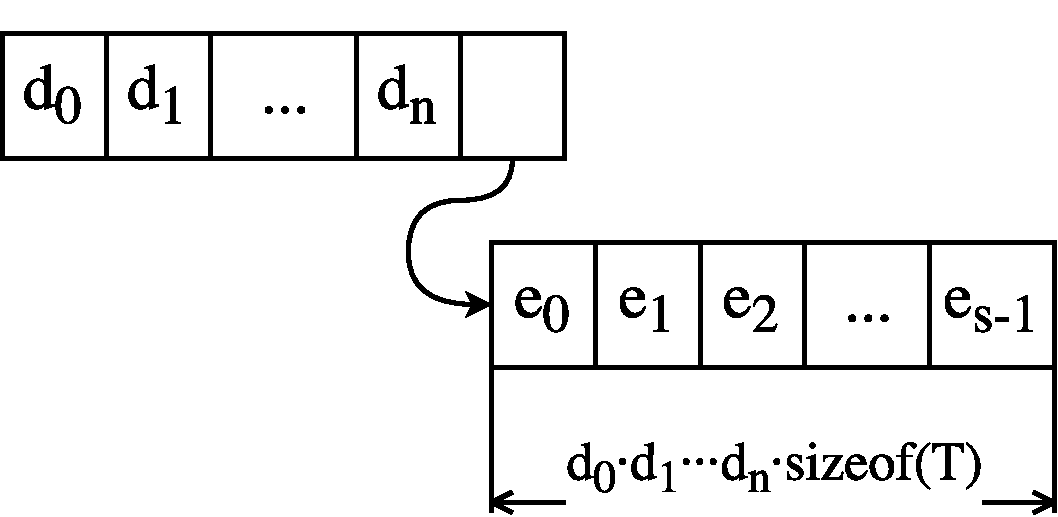
\includegraphics[width=0.5\textwidth]{diag2}}
    \label{fig:diag}
\end{figure}

Cuando todas las dimensiones del arreglo son conocidas a tiempo de compilación,
los tamaños de cada dimensión son almacenados estáticamente en la <<cabecera>> y
se reserva el espacio para los elementos en el tipo de memoria apropiado. Cuando
este no es el caso, se genera el código para, a tiempo de ejecución, evaluar la
expresión correspondiente a cada dimensión del arreglo, almacenar en el campo
correspondiente de la cabecera el valor resultante, y reservar el espacio para
los elementos en el tipo de memoria apropiado.

El hecho de que sean almacenados en dos partes podría causar preocupaciones
respecto a la liberación de memoria ocupada por arreglos dinámicos. Sin embargo,
este caso fue tomado en cuenta y la liberación de memoria procede en dos partes,
liberando primero el bloque de elementos, y posteriormente la <<cabecera>>.

La última consideración sobre los arreglos está asociada con su uso como
parámetros de subrutinas (procedimientos y funciones). Se agregó al lenguaje la
capacidad para usar arreglos como parámetros de los modos In, In-Out y Out,
además del modo Ref ya provisto en la especificación original. Adicionalmente,
se decidió permitir el pase de arreglos de tamaño arbitrario como parámetros
siempre que todas las variables en las expresiones que denotan su tamaño sean
parámetros anteriores de la subrutina, pasados en modo \ingra{const} en el caso
de los procedimientos. Por ejemplo, la firma de procedimiento en el fragmento de código~\ref{lst:arrproc} sería
aceptada por el compilador:

\begin{gracielacode}[caption=Firma de procedimiento con parámetro de tipo arreglo, label=lst:arrproc]
proc sub(
  const size : int,
  inout arr : array [size, size * 2] of int
)
\end{gracielacode}

Desafortunadamente, un procedimiento (o una función) con una firma similar a la
de \ingra{sub} podría ser llamado con argumentos que no concuerden, como en el
fragmento de código~\ref{lst:arrproccall}.

\begin{gracielacode}[caption=Llamada a procedimiento con argumento de tipo arreglo, label=lst:arrproccall]
|[ var arr : array [5, 5]
 ; sub (5, arr)
]|
\end{gracielacode}

En este caso, el procedimiento \ingra{sub} espera un arreglo de tamaño
\ingra{[size, (size * 2)]}, y como recibe \ingra{size = 5}, espera que el tamaño
del arreglo sea \ingra{[5, 1~~0]}. Sin embargo, recibe un arreglo de tamaño
\ingra{[5, 5]}, por lo cual la ejecución debe abortar al momento de esa llamada.
Esta verificación no puede hacerse a tiempo de compilación en el caso general,
puesto que sería equivalente a predecir todos los posibles cursos de ejecución
del programa.

%%%%%%%%%%%%%%%%%%%%%%%%%%%%%%%%%%%%%%%%%%%%%%%%%%%%%%%%%%%%%%%%%%%%%%%%%%%%%%%%
\subsection{Consideraciones sobre funciones y procedimientos}

Se decidió cambiar ligeramente la gramática de las funciones y procedimientos
para que fueran más similares a sus equivalentes en GCL. Simplemente, se
eliminaron los lexemas \ingra{begin} y \ingra{end}, antes usados para
delimitar el procedimiento, y el lexema \ingra{:} entre el identificador de la
subrutina y su lista de parámetros, y se movió la postcondición junto a la
precondición, antes del cuerpo de la subrutina.

Además, se agregó la posibilidad de especificar cotas para las subrutinas luego
de la postcondición y antes del cuerpo, como requisito para hacer llamadas
recursivas dentro de la misma. Así, es un error a tiempo de compilación escribir
una llamada recursiva de una subrutina sin cota. En el caso contrario, el de una
subrutina con cota pero sin recursión, ésta simplemente es ignorada. A pesar de
que esto no estaba dentro de los objetivos de este proyecto, se consideró de
suma importancia, puesto que la recursión sin cotas es equivalente a la
iteración sin cotas, prohibida en el caso de la instrucción \ingra{do .. od}.

El código intermedio LLVM generado para una subrutina recursiva, necesariamente
con cota, además de incluir el cuerpo especificado por el programador, incluye
verificaciones para el decrecimiento y la no-negatividad de la cota. Esto se
logra pasando dos parámetros adicionales a las subrutinas recursivas. El
primero, de tipo booleano, indica si la llamada en curso es la primera llamada a
la subrutina o si se trata de una llamada recursiva. En ambos casos, al entrar a
la subrutina se calcula el valor de la cota, y si es negativa se da un error y
el programa aborta. En caso contrario, si se trata de la primera llamada a la
subrutina, se ejecuta el cuerpo de ésta, pero si se trata de una llamada
recursiva, se compara la cota actual con la anterior, recibida como el segundo
parámetro implícito. Si no hubo decremento en la cota, también se da un error y
el programa aborta. En caso contrario, se ejecuta el cuerpo de la subrutina.

Por último, cabe mencionar que se cambió la semántica del modo de parámetros
\ingra{in}, de forma que los parámetros declarados con este modo pueden ser
reasignados dentro del cuerpo del procedimiento sin afectar el valor del
argumento usado en el punto de llamada. Originalmente, los parámetros de modo
\ingra{in} no podían ser reasignados, pero se consideró que sería conveniente
poder reasignarlos para ofrecer la posibilidad de usar parámetros por su valor
pero aprovechando su espacio en memoria. El comportamiento asociado
anteriormente al modo \ingra{in} ahora corresponde al modo de parámetros
\ingra{const}.

%%%%%%%%%%%%%%%%%%%%%%%%%%%%%%%%%%%%%%%%%%%%%%%%%%%%%%%%%%%%%%%%%%%%%%%%%%%%%%%%
\subsection{Consideraciones sobre cuantificaciones}

Durante el análisis del compilador original, se conoció que las cuantificaciones
presentaban limitaciones en la expresividad de sus rangos. El analizador
sintáctico de esta parte del lenguaje esperaba, específicamente, dos
comparaciones aritméticas, separadas por un operador de conjunción
(\ingra{/\}), seguidas por un lexema <<barra vertical>>
(\ingra{|}). Esto impedía expresar condiciones lógicas distintas de
comparaciones aritméticas, como predicados definidos por el programador, o
incluso condiciones con más de dos comparaciones aritméticas.

Para solucionar esto, se agregó un estado al analizador sintáctico de las
expresiones, usando el \emph{Monad Transformer} \ingra{StateT} sobre el
\emph{Monad} \ingra{Parsec}. En este estado, se guarda información sobre la
pila de variables generadora presentes en un momento dado (la pila vacía en el
caso de las expresiones sin cuantificaciones). Además, se permitió que el
analizador sintáctico de las expresiones devolviera, además de la expresión
conseguida, el rango asociado a ella. Por ejemplo, con la variable generadora
\ingra{x}, la expresión \ingra{x >= 5} tiene asociado el rango $[5, \infty)$.

Cuando el analizador sintáctico se encuentra en una cuantificación, agrega la
variable generadora correspondiente a la pila del estado, e intenta construir un
rango. Los únicos operadores que construyen rangos son la igualdad (\ingra{==}),
que construye rangos <<unitarios>>; las comparaciones aritméticas (\ingra{>},
\ingra{>=}, \ingra{<}, \ingra{<=}), que construyen rangos <<aritméticos>>; y el
operador <<pertenece>> de la Teoría de Conjuntos ($\in$) [ver sección
\ref{sect:sets}], que produce rangos <<conjunto>>, mientras que la constante
booleana \ingra{false} produce el rango <<vacío>>.

Además, el operador de conjunción (\ingra{/\}) devuelve, si es
posible, el rango que resulta de intersectar los rangos asociados a cada uno de
sus operandos. A diferencia de las cuantificaciones lógicas, sin embargo, no se
consideran los rangos generados por el operador de disyunción
(\ingra{\/}), por lo cual si se desea que un rango sea procesado
como tal, debe estar escrito en Forma Normal Conjuntiva. Esto no le resta
expresividad al lenguaje, ya que pueden conseguirse expresiones equivalentes con
el uso de teoremas lógicos, convirtiendo una cuantificación en la disyunción de
varias, o usando el operador de unión de conjuntos (\ingra{~\Union~}).

Finalmente, si se ha construido un rango válido, este se registra en el ASA
correspondiente a la cuantificación. Si el rango es <<aritmético>>, se exige que
existan límites superior e inferior, emitiéndose el error apropiado en caso de
faltar uno de los límites. Cabe mencionar que si la variable generadora es de
tipo número de punto flotante, las comparaciones aritméticas \emph{no} generarán
rangos, puesto que no existe una manera obvia de iterar sobre números de este
tipo.

El código intermedio LLVM generado para cada cuantificación dependerá de la
clase del rango sobre el cual esté definida:

\begin{description}

  \item [Rango <<vacío>>] se genera el valor neutro del cuantificador, o, en el
caso de los cuantificadores \ingra{max} y \ingra{min}, una llamada al mensaje
de error apropiado.

  \item [Rango <<unitario>>] se genera el código del cuerpo de la cuantificación
con la sustitución apropiada de la variable generadora.

  \item [Rango <<aritmético>>] se genera una iteración en la cual la variable
generadora toma todos los valores entre el límite inferior y el superior, y se
evalúa el cuerpo, acumulando los resultados. Existe la posibilidad de que a
tiempo de ejecución esto resulte en un rango vacío, y en este caso el
comportamiento es el esperado, pues la iteración es vacía.

  \item [Rango <<conjunto>>] se genera una iteración en la cual la variable
generadora toma todos los valores pertenecientes al conjunto (o multiconjunto,
o secuencia), y se evalúa el cuerpo, acumulando los resultados. En el caso de un
rango secuencia, el orden de la iteración es el mismo de la secuencia, mientras
que para conjuntos y multiconjuntos no se garantiza ningún orden en particular.
De nuevo, es posible que un rango de esta clase resulte en un rango vacío a
tiempo de ejecución, pero el comportamiento sigue siendo el esperado.

\end{description}


%%%%%%%%%%%%%%%%%%%%%%%%%%%%%%%%%%%%%%%%%%%%%%%%%%%%%%%%%%%%%%%%%%%%%%%%%%%%%%%%
%% TEORÍA DE CONJUNTOS %%%%%%%%%%%%%%%%%%%%%%%%%%%%%%%%%%%%%%%%%%%%%%%%%%%%%%%%%
%%%%%%%%%%%%%%%%%%%%%%%%%%%%%%%%%%%%%%%%%%%%%%%%%%%%%%%%%%%%%%%%%%%%%%%%%%%%%%%%
\section{Teoría de conjuntos}\label{sect:sets}
\subsection{Consideraciones}

Para permitir mayor expresividad en las aserciones del lenguaje, específicamente
en aquellas asociadas con los tipos de dato definidos por el programador, como
invariantes de representación y de acoplamiento, se decidió agregar al lenguaje
Graciela facilidades para escribir expresiones de la teoría de conjuntos.
Específicamente, se consideró necesario agregar los tipos conjunto,
multiconjunto, secuencia, función y relación. En adelante, se usará el término
\textit{colección} para hablar indistintamente de conjuntos, multiconjuntos y
secuencias.

El primer obstáculo encontrado fue el uso ligero de la notación en la literatura
para la representación de conjuntos y multiconjuntos. En general, se usa para
ellos la misma notación, y la distinción entre ambos tipos se hace según el
contexto. Como es posible que en un programa escrito en Graciela haga uso de
ambos tipos de colección, la forma más directa de distinguirlos fue usar
notación distinta para cada uno. Se decidió entonces usar los símbolos \ingra|{|
y \ingra|}| para los conjuntos y \Lbag{} y \Rbag{} para los multiconjuntos si se
usan caracteres UTF-8  o \ingra|{:| y \ingra|:}| si no. Similarmente, como no
existe una notación estándar para las secuencias, se decidió usar los símbolos
\Lseq{} y \Rseq{} si se usan caracteres UTF-8 o \ingra|<<| y \ingra|>>| si no.

En segundo lugar, se observó que debían incluirse dos maneras de definir
colecciones, por su uso en los cursos teóricos de algorítmica, las definiciones
por extensión y por comprensión.

Para las definiciones por extensión, el análisis sintáctico consiste simplemente
en reconocer el símbolo de apertura correspondiente a la colección y luego una
secuencia potencialmente vacía de expresiones de un mismo tipo separadas por
comas, y finalmente el símbolo de cierre apropiado. El código generado para
estas colecciones no es más que la adición iterada de cada elemento sobre una
colección inicialmente vacía.

Para las definiciones por comprensión, se observó la similitud entre esta
notación y la de las cuantificaciones, y se aprovecharon parcialmente los
reconocedores de estas últimas. Específicamente, una colección por comprensión
consta de tres partes separadas por símbolos \ingra{|} entre los símbolos
correspondientes a la colección. En la primera parte, se define una variable
auxiliar con su tipo, en la segunda se define un rango para la variable, con las
mismas consideraciones que para las cuantificaciones, y en la última, el cuerpo,
aparece la expresión que será agregada a la colección para cada elemento del
rango. El código generado para este caso es precisamente la iteración sobre el
rango, donde cada vez se evalúa la expresión del cuerpo y se agrega a una
colección inicialmente vacía.

Cabe mencionar que sólo se permiten colecciones de un nivel, es decir, no se
permiten colecciones de colecciones, sino únicamente colecciones de tipos
básicos (\ingra{int}, \ingra{char}, \ingra{float}, \ingra{boolean}) o de pares
ordenados de tipos básicos.

Para las funciones y relaciones también se encontró un problema al definir una
notación. En la literatura, ambos tipos son representados como conjuntos de
pares ordenados, y se distingue entre ellos según el contexto. Para evitar
conversiones implícitas entre tipos que representan conceptos diferentes, se
optó por definir las funciones \ingra{func} y \ingra{rel}, que toman un conjunto
de pares ordenados (\ingra{A}, \ingra{B}), donde \ingra{A} y \ingra{B} son tipos
básicos posiblemente distintos, y devuelven, respectivamente, la función de
\ingra{A} en \ingra{B} y la relación entre \ingra{A} y \ingra{B}
correspondientes al conjunto de pares dado. El código intermedio generado para
la función \ingra{func} verifica que no existan pares con el mismo primer
elemento y convierte internamente el conjunto de pares en un \texttt{Map} (de la
biblioteca estándar de C++) entre los tipos apropiados, mientras que para la
función \ingra{rel} no es necesario generar código.

También se extendió la notación de llamada de funciones para soportar funciones
y relaciones en su sentido matemático. Para esto, fue necesario convertir los
paréntesis en un operador posfijo dentro de la gramática de las expresiones, a
diferencia de su definición en la gramática original como un identificador
seguido de un paréntesis, puesto que ahora es posible llamar funciones (y
relaciones) anónimas escritas con \ingra{func} y \ingra{rel} a partir de
conjuntos. Similarmente, se extendió la notación de indización de arreglos para
soportar secuencias, dado que también es posible indizar secuencias anónimas
definidas por extensión o por comprensión.

Adicionalmente, fue necesario permitir la declaración de variables de tipos
colección, función y relación, pero únicamente dentro de Tipos de Dato
Abstractos, por lo cual se agregó al analizador sintáctico para declaraciones la
capacidad de reconocer estos tipos y de dar mensajes de error apropiados cuando
se intente usarlos fuera de Tipos de Dato Abstractos.

Finalmente, se agregaron los operadores usuales de la teoría de conjuntos. Se
hace una exposición de ellos en el apéndice NUMERODEAPENDICE.

\subsection{Biblioteca externa para teoría de conjuntos}

Internamente, los valores de la teoría de conjuntos son manejados como
apuntadores a las estructuras correspondientes ofrecidas por la biblioteca
estándar del lenguaje C++. Esto se hace de manera transparente al programador,
por lo cual éste no debe preocuparse por manejar dichos apuntadores. Como  estas
estructuras se crean de manera dinámica y su manejo es responsabilidad del
compilador y de la biblioteca externa, se diseñó un sencillo manejador de
memoria dinámica que libera el espacio asignado a dichas estructuras cada vez
que salen de alcance. Si el programa termina de manera inesperada por haberse
incumplido una aserción, o por haber alcanzado un condicional sin guardas
verdaderas, este manejador de memoria se encarga de liberar toda la memoria
reservada para estas estructuras.


%%%%%%%%%%%%%%%%%%%%%%%%%%%%%%%%%%%%%%%%%%%%%%%%%%%%%%%%%%%%%%%%%%%%%%%%%%%%%%%%
%% MANEJO DE APUNTADORES %%%%%%%%%%%%%%%%%%%%%%%%%%%%%%%%%%%%%%%%%%%%%%%%%%%%%%%
%%%%%%%%%%%%%%%%%%%%%%%%%%%%%%%%%%%%%%%%%%%%%%%%%%%%%%%%%%%%%%%%%%%%%%%%%%%%%%%%
\section{Manejo de apuntadores}

\subsection{Consideraciones}
Los apuntador implementados para el lenguaje Graciela pueden apuntar a un
objeto cualquier tipo básico, arreglo o tipo definido por el programador. La
sintaxis para declarar un apuntador es parecida a la presente en  el lenguaje
C, es decir, se escribe el tipo base seguido de tantos asteriscos (\ingra{*})
como apuntadores se desee. El operador para acceder a la memoria apuntada por
un apuntador es igualmente el asterisco, el cual debe colocarse como operador
prefijo a una expresión de tipo apuntador.

La reserva y liberación de memoria dinámica para un apuntador se realiza con las
funciones propias del lenguaje \ingra{new} y \ingra{free}, ambas con
consideraciones adicionales para el caso de apuntadores a arreglos y apuntadores
a tipos definidos por el programador, que se describen detalladamente en sus
respectivas secciones. El fragmento de código~\ref{lst:point} ejemplifica la
declaración y uso de un apuntador a entero.

\begin{gracielacode}[caption=Uso de apuntadores, label=lst:point]
|[ var p : int *
 ;  new(p)
 ;  *p := 10
 ;  free(p)
]|
\end{gracielacode}

\subsection{Generación de código intermedio}

LLVM ofrece un soporte completo para el manejo de apuntadores, lo que facilitó
enormemente la tarea de implementar la generación de código intermedio para el
manejo de apuntadores. Sin embargo, carece de instrucciones para la reserva y
liberación de memoria dinámica, razón por la cual hubo la necesidad de colocar
funciones en la biblioteca externa que recibieran como argumento al apuntador en
cuestión, y que a su vez llamaran rutinas del lenguaje C que se ocupasen de
realizar dichas operaciones.

En el momento en que se crea un apuntador, éste se inicializa con un valor nulo,
evitando así poder acceder a una dirección basura. En caso de tratar acceder a
la memoria apuntada por un apuntador que contenga la dirección nula, se emite un
error a tiempo de ejecución que indica el lugar de dicho acceso, impidiendo que
sea el sistema operativo quien emita el error.

Para la reserva de memoria dinámica, se utilizó la función estándar de C
\texttt{calloc}, la cual reserva la cantidad de memoria que se le da como
argumentos e inicializa todos los bytes a $0$. Por otro lado, la liberación de
memoria dinámica se realiza llamando a la función estándar de C \texttt{free}.

\subsection{Lógica de Separación}

Durante la etapa de planificación y diseño de la extensión al lenguaje Graciela,
se consideró la posibilidad de agregar a este el soporte para expresiones
propias de la lógica de separación, de modo que los programadores pudieran
especificar de manera sencilla propiedades acerca de estructuras recursivas que
hicieran uso de apuntadores. Sin embargo, para implementar los operadores
propios de la lógica de separación, $*$ (conjunción separadora), $\mapsto$
(deconstrucción de \textit{heap} unitario), y $-*$ (implicación separadora), así
como la constante $emp$, es necesario almacenar la información correspondiente
al \textit{heap} en cada caso, exigiendo el manejo cuidadoso a tiempo de
ejecución de estructuras internas temporales con este fin.

Debido a esta dificultad, se decidió no agregar expresiones de la lógica de
separación al lenguaje, y en su lugar ofrecer la alternativa más sencilla de
comparar apuntadores con el operador de igualdad, \ingra{==}. Otro factor que
influyó en esta decisión fue la consideración de que el público para el cual
está dirigido el lenguaje Graciela, los estudiantes de los cursos introductorios
de algoritmos y estructuras, tan sólo está familiarizado con la lógica de
predicados, y está estudiando la lógica de Hoare, por lo cual agregar a esta
carga otro sistema formal (uno que no pertenece a los programas de
estudios de los cursos en cuestión) resultaría en un gran potencial para
confusión para el programador, sin agregar mucho valor al lenguaje.


%%%%%%%%%%%%%%%%%%%%%%%%%%%%%%%%%%%%%%%%%%%%%%%%%%%%%%%%%%%%%%%%%%%%%%%%%%%%%%%%
%% TIPOS DE DATO (...) %%%%%%%%%%%%%%%%%%%%%%%%%%%%%%%%%%%%%%%%%%%%%%%%%%%%%%%%
%%%%%%%%%%%%%%%%%%%%%%%%%%%%%%%%%%%%%%%%%%%%%%%%%%%%%%%%%%%%%%%%%%%%%%%%%%%%%%%%
\section{Tipos de dato definidos por el programador}

%  - LA GRAMÁTICA VA AL FINAL PERO IGUAL HABLAMOS SOBRE ELLA -> SOBRE TODO EL WHERE

\subsection{Consideraciones}
% - Consideraciones

El objetivo principal de este proyecto es agregar al lenguaje Graciela y a su
compilador, las características y el soporte necesarios para permitir al
programador definir tipos de dato estructurados abstractos o TDA. Como se busca
lograr que el lenguaje Graciela cuente con la misma expresividad del lenguaje
GCL, es necesario que su compilador permita definir restricciones y
comportamientos abstractos para estos tipos, a través del uso de aserciones de
alto nivel como el invariante de representación y las precondiciones y
postcondiciones de los procedimientos y funciones que definen su interfaz.
Estos tipos de dato, definidos dentro del lenguaje de programación con la
palabra reservada \ingra{abstract}, nunca definen una implementación en
particular, sino que se limitan, precisamente, a definir los comportamientos que
debería cumplir cualquier estructura de datos que pretenda implementarlos.

Para aprovechar la definición de un tipo de dato abstracto, es necesario definir
un nuevo tipo de dato que, usando únicamente estructuras de bajo nivel y un
invariante de acoplamiento que precise la correspondencia entre estas
estructuras de bajo nivel y las de alto nivel del tipo de dato abstracto, logre
cumplir las restricciones y comportamientos de este último. En adelante, nos
referiremos a estos tipos de dato, los cuales siempre deben implementar un TDA,
como \textit{implementaciones}. Dentro del lenguaje, estos son definidos usando
la palabra reservada \ingra{type} y el TDA implementado se especifica usando la
palabra reservada \ingra{implements}.

Sin embargo, en el caso general, no es posible verificar, a tiempo de
compilación, que una implementación de un tipo de dato, junto con sus
procedimientos y funciones, cumpla a cabalidad con los invariantes y aserciones
del tipo de dato abstracto que se supone implementa. Por lo tanto, se decidió
dejar algunas de estas verificaciones para tiempo de ejecución.

\subsection{Modelo de representación}

Dentro de un tipo de datos se pueden declarar variables y constantes, a los
cuales puede darse un valor inicial en caso de ser de un tipo básico o
apuntador. Estas declaraciones corresponden al modelo de representación del tipo
de dato. Si se trata de un TDA, se pueden declarar variables con un tipo de alto
nivel, es decir, tipos de la Teoría de Conjuntos.

A nivel del código generado, se consideró la posibilidad de mantener estas
variables actualizadas según se ejecuten los distintos procedimientos del TDA,
con cada instrucción produciendo, posiblemente, varias actualizaciones sobre
estas estructuras, en general difíciles de predecir. Inclusive, el código que
manipulara directamente la \textit{implementación} del TDA, fuera de sus
procedimientos, debería ser capaz de actualizar estas estructuras, ya que de lo
contrario se producirían inconsistencias. Así, se optó por no almacenar de
manera persistente las variables del TDA de tipos de la teoría de conjuntos,
sino por materializarlas, haciendo uso de la relación de acoplamiento, sólo
cuando son necesarias para evaluar las distintas aserciones del TDA, por
ejemplo, al momento de evaluar las precondiciones y postcondiciones de un
procedimiento abstracto.

\subsection{Invariante de representación}

El invariante de representación define las características y restricciones que
deben ser satisfechas por el modelo de representación de un tipo de dato, sea un
TDA o una implementación de un TDA. El invariante de representación se indica
como una expresión booleana contenida entre el par de símbolos \ingra|{repinv|
y \ingra|repinv}|. Es importante destacar que, en el caso de las
implementaciones, las variables y constantes del TDA implementado pueden ser
utilizadas dentro del invariante de representación, siempre y cuando no sean de
tipos de la Teoría de Conjuntos.

\subsection{Relación de acoplamiento}

En la literatura, para establecer la relación entre las estructuras de bajo
nivel usadas en la implementación, con las de alto nivel que se encuentran en el
TDA, es decir, se debe definir una correspondencia entre los dos modelos de
representación en la forma de una expresión lógica arbitraria. Como se explica
en la sección anterior sobre el modelo de representación, se decidió que las
estructuras de tipos de la teoría de conjuntos sólo fueran materializadas al
momento de verificar aserciones. Por lo tanto, es necesario contar con
instrucciones para materializarlas. Sin embargo, las expresiones lógicas
arbitrarias no proveen una manera directa para generar dichas instrucciones,
puesto que la lógica declarativa únicamente especifica propiedades, y deducir
valores a partir de estas propiedades, en el caso general, resulta imposible,
puesto que más de un valor podría satisfacer dicho conjunto de propiedades. Se
notó, a pesar de esto, que la mayoría de las relaciones de acoplamiento
encontradas en la literatura tenían una estructura particular: consistían de
igualdades con un sólo término a la izquierda, unidas por conjunciones. En las
demás,  se notó que podían ser reescritas para cumplirla, o al menos como una
conjunción donde al menos un conjuntor la cumple.

Debido a estas consideraciones, se decidió separar la escritura de la relación
de acoplamiento en dos partes: una serie de asignaciones que definen las
estructuras de la teoría de conjuntos, en las cuales se puede hacer uso de la
sintaxis incorporada al lenguaje para la construcción de expresiones de este
tipo, ubicadas dentro de un bloque  precedido por la palabra reservada
\ingra{where}, a la cual nos referiremos en adelante como \textit{la}
<<relación de acoplamiento>>, y una expresión lógica con las restricciones
usuales de estas expresiones para especificar el resto de las propiedades del
acoplamiento, escrita entre los símbolos \ingra|{coupinv| y
\ingra|coupinv}|, a la cual nos referiremos en adelante como el <<invariante
de acoplamiento>>.

\subsection{Variables de tipo}

En el lenguaje GCL es posible especificar tipos de dato estructurados que no
dependen de tipos concretos para sus operaciones. Por ejemplo, se puede definir
el tipo \textit{Lista} sin  especificar, en la definición, si se trata de listas
de enteros o de números de punto flotante. Como se desea que el lenguaje
Graciela cuente con la misma expresividad de GCL, es necesario poder hacer esto.
Para ello se dotó al lenguaje con la capacidad de permitir la declaración de
tipos genéricos que permiten definir aserciones y comportamientos igualmente
genéricos.

Estos tipos genéricos, o variables de tipo, se pueden declarar junto con la
definición de un tipo de dato y usarse en la especificación interna de éste. Las
variables de tipos solo pueden ser sustituidas por un tipo básico, es decir,
tipo entero, flotante, carácter o booleano. Al momento de
declarar una variable de un tipo de dato definido por el programador con
variables de tipo asociadas, se deben  especificar los tipos básicos que
correspondan a cada variable en cuestión. Un ejemplo de esto puede verse en el
fragmento de código~\ref{lst:insttvar}.

\begin{gracielacode}[caption=Instanciación de variables de tipo, label=lst:insttvar]
abstract ConjuntoA (T) begin
  var a : T;
  ...
end

type Conjunto (N) implements ConjuntoA (N) begin
  var b : N;
  ...
end

main
 |[ var c : Conjunto (int)
    ...
 ]|
\end{gracielacode}

En este caso, se definió un tipo de dato abstracto \ingra{ConjuntoA} y una
implementación \ingra{Conjunto}, ambas haciendo uso de variables de tipo,
\ingra{T} y \ingra{N} respectivamente. Como se puede apreciar, el tipo
\ingra{Conjunto} implementa el TDA \ingra{ConjuntoA} con la variable de tipo
\ingra{N} sustituyendo a la variable de tipo \ingra{T}, por lo que cada
ocurrencia de \ingra{T} dentro de la especificación de \ingra{ConjuntoA}, será
sustituida por la variable de tipo \ingra{N}.

Por otro lado, cuando se declara la variable \ingra{c}, es necesario indicar un
tipo concreto, en este caso \ingra{int}, para el tipo \ingra{Conjunto}. De
esta forma cualquier ocurrencia de \ingra{N} (incluyendo las ocurrencias de
\ingra{T} en \ingra{ConjuntoA} sustituidas en el paso anterior), dentro de la
especificación de \ingra{Conjunto}, es sustituida por el tipo \ingra{int}.

\subsection{Procedimientos y funciones}

Como se mencionó previamente, los tipos de dato abstractos definen una
interfaz. Esta interfaz se compone de una serie de procedimientos y funciones,
cada una con sus respectivas precondiciones y postcondiciones.

Para definir una implementación de un tipo abstracto, se debe definir la
implementación de todos los procedimientos y funciones que se encuentran en la
interfaz del TDA, junto con un nuevo par de precondiciones y postcondiciones que
podrán referirse únicamente a las estructuras propias de la implementación.
Adicionalmente, una implementación puede agregar procedimientos y funciones que
no estén presentes en el TDA implementado.

Cabe mencionar las siguientes consideraciones:

\begin{itemize}

  \item Si una subrutina hace uso de una variable de tipo, es necesario que al
  menos uno de sus parámetros sea del tipo de dato dentro del cual se define
  dicha subrutina.

  \item Dentro de un tipo de dato, cada subrutina debe tener un nombre único.
  Sin embargo, ese nombre puede ser reutilizado en otro tipo de dato, siempre y
  cuando uno de sus parámetros sea del tipo de dato en cuestión. Al momento de
  decidir cuál subrutina se debe escoger, el compilador toma el primer
  argumento, de izquierda a derecha, cuyo tipo sea un tipo de dato definido por
  el usuario, para escoger la subrutina apropiada. En caso de haber más de una
  subrutina que cumpla esta condición, se toma como un caso ambiguo y se emite
  un error a tiempo de compilación.

\end{itemize}

\subsection{Generación de código intermedio}

Durante el análisis sintáctico, se registran todos los usos de un tipo de dato
definido por el programador, y los diferentes tipos concretos que se les asigna
en cada uso. De esta forma, para un tipo \ingra{Diccionario(T0, T1)}, se guarda
la información sobre sus apariciones en declaraciones y los tipos básicos usados
en cada una. Si los usos fueron \ingra{Diccionario(int, char)} y
\ingra{Diccionario(int, float)}, al llegar a la fase de generación de código
intermedio, se generan dos estructuras de bajo nivel con el nombre del tipo en
cuestión seguido de las iniciales de los tipos básicos utilizados separados por
guiones, es decir, \texttt{Diccionario-i-c} y \texttt{Diccionario-i-f}, ambas
conteniendo los campos de la implementación y del TDA. Cabe destacar que nunca
se generan estructuras en el código intermedio para los TDA.

Es necesario destacar sobre los arreglos, que al estar separados en una cabecera
y un cuerpo, solo la cabecera es incluida dentro de la estructura. El cuerpo es
almacenado en una parte separada de la memoria, en la pila en caso de ser una
variable estática, o en memoria dinámica en caso de tratarse de un apuntador.

\subsubsection{Invariantes de representación y de acoplamiento}

Por cada estructura generada para cada tipo de dato, se generan automáticamente
tres subrutinas, a saber, una para el invariante de representación del TDA,  una
para el invariante de representación de la implementación, y una para la
relación de acoplamiento. Estas rutinas serán llamadas repetidamente dentro de
las verificaciones de cada procedimiento y función dentro del tipo de dato. De
esta manera, se evita repetir en el código intermedio generado las instrucciones
asociadas a invariantes de representación y relaciones de acoplamiento.

\subsubsection{Procedimientos y funciones}

Para los procedimientos y funciones debemos considerar dos casos. Si la
subrutina no hace uso alguno de variables de tipo, se genera una única rutina en
código intermedio. En el caso contrario, se generan tantas rutinas en código
intermedio como estructuras del tipo de dato en cuestión se hayan generado. De
esta forma, suponiendo que el procedimiento \ingra{agregar} del tipo
\ingra{Conjunto(T)} tiene un parámetro de tipo \ingra{Conjunto(T)}, y que en
el código principal del programa se declararon variables de los tipos
\ingra{Conjunto(int)} y \ingra{Conjunto(char)}, serán generadas en el código
intermedio dos subrutinas llamadas \texttt{agregar-Conjunto-i} y
\texttt{agregar-Conjunto-c}.

Con respecto a la verificación de las precondiciones, postcondiciones e
invariantes, se genera el código necesario para las siguientes verificaciones:

\begin{enumerate}

  \item Antes de iniciar el cuerpo del procedimiento, se evalúa la precondición
  de la implementación. En caso de ser falsa, se emite una advertencia a tiempo
  de ejecución y no se hacen más verificaciones.

  \item Si la precondición se cumple, se utiliza la relación de acoplamiento
  apropiada para materializar las estructuras de los TDAs correspondientes a
  parámetros de tipos definidos por el programador, y se verifica cada invariante
  de acoplamiento. En caso de que alguno de estos sea falso, se emite un error a
  tiempo de ejecución.

  \item Para cada parámetro de tipo definido por el programador, se verifica
  el invariante de representación de la \textit{implementación} correspondiente.
  Si alguno de estos es falso, se emite un error a tiempo de ejecución.

  \item En el caso de los procedimientos que implementan procedimientos del TDA,
  en este punto se evalúa la precondición de este último. Si esta es falsa, se
  emite un error a tiempo de ejecución, aclarando que el procedimiento no
  implementa el procedimiento correspondiente del TDA. Si no existe un procedimiento
  correspondiente en el TDA, es decir, si se trata bien de un procedimiento
  definido únicamente en la \textit{implementación} del tipo, o bien de un
  procedimiento definido en el espacio global de definiciones, esta verificación
  es omitida.

  \item Para cada parámetro de un tipo definido por el programador, se verifica
  el invariante de representación del TDA correspondiente. Si alguno de estos es
  falso, se emite un error a tiempo de ejecución.

  \item En este punto, si todas las verificaciones anteriores han sido exitosas,
  se procede a ejecutar el cuerpo del procedimiento.

  \item Finalizado el cuerpo del procedimiento, se aplica nuevamente la relación
  de acoplamiento de cada parámetro de tipo definido por el programador, y se
  verifica cada invariante de acoplamiento. En caso de que alguno de estos sea
  falso, se emite un error a tiempo de ejecución.

  \item Para cada parámetro de tipo definido por el programador, se verifica el
  invariante de representación del TDA correspondiente. Si alguno de estos es
  falso, se emite un error a tiempo de ejecución.

  \item En el caso de los procedimientos que implementan
  procedimientos del TDA, en este punto se evalúa la postcondición de este
  último. Si esta es falsa, se espera a la verificación de la postcondición de la
  implementación para emitir el error apropiado. Si es verdadera, continúan las
  demás verificaciones de esta lista. Si no existe un procedimiento
  correspondiente en el TDA, es decir, si se trata bien de un procedimiento
  definido únicamente en la \textit{implementación} del tipo, o bien de un
  procedimiento definido en el espacio global de definiciones, esta verificación
  es omitida.

  \item Para cada parámetro de tipo definido por el programador, se verifica el
  invariante de representación de la \textit{implementación} correspondiente. Si
  alguno de estos es falso, se emite un error a tiempo de ejecución.

  \item Por último, se evalúa la postcondición de la \textit{implementación}. En
  este punto, el curso del programa dependerá de los valores que hayan tomado
  esta última y la postcondición del TDA. Si no existe un procedimiento
  correspondiente en el TDA, se toma su valor como verdadero.
    \begin{itemize}
      \item Si se cumplieron ambas postcondiciones, la ejecución sigue normalmente
      \item Si sólo se cumple la postcondición del la implementación, se emite el
      error <<No se cumple la postcondición>>
      \item Si sólo se cumple la postcondición del TDA, se emite el error <<Este
      procedimiento no implementa el TDA>>
      \item Si ninguna de las dos postcondiciones se cumple, se emiten ambos errores.
    \end{itemize}
\end{enumerate}

Estas consideraciones aplican para las funciones, con la excepción de los
invariantes, que no se verifican por segunda vez al salir de la función. Esto se
debe a que son funciones puras y por lo tanto, no realizan cambios en las
variables involucradas.

\subsubsection{Otras rutinas creadas implícitamente}

Para cada estructura creada a partir de un tipo de dato definido por el programador,
se generan automáticamente un constructor, un destructor y una rutina para la
copia de las estructuras. Las siguientes consideraciones son contempladas para
estas rutinas:

\begin{itemize}

  \item El constructor es llamado cuando se declara una variable del tipo en
  cuestión, o después de haber reservado memoria para un apuntador del mismo
  tipo. Esta rutina se encarga de asignar a cada campo de la estructura el
  valor inicial que corresponda, reservar espacio en memoria para la cabecera
  y el cuerpo de los campos de tipo arreglo y llamar recursivamente a los
  constructores de las estructuras internas, si las hubiera.

  \item La rutina de copia se utiliza para copiar la estructura cuando se
  intenta pasar como argumento In o In-Out a un procedimiento. La copia se hace
  de manera superficial cuando se trata de apuntadores; es decir, se copia la
  dirección contenida en el apuntador y no la estructura apuntada.

  \item Antes de liberar un apuntador hacia una estructura, se llama al
  destructor, el cual se encarga de liberar la memoria reservada por el cuerpo
  de la estructura, luego de llamar recursivamente a los destructores de las
  estructuras internas. El destructor no libera la memoria apuntada por campos
  de tipo apuntador.

\end{itemize}

% TDDDPEU
% Variables de tipo
% - Invariantes de representación, acoplamiento
%     - Invariante de acoplamiento "compilable"
% - Procedimientos y Funciones de/sobre un TDA
% - Funciones predefinidas (inicializador y destructor)

\subsection{Verificación de tipos}

Para poder integrar los tipos de dato definidos por el programador al sistema
de tipos del compilador de Graciela, fue necesario extender el verificador de
tipos. Esto se hizo definiendo un monoide sobre el conjunto de los tipos de
Graciela, con el elemento neutro <<cualquier tipo>>, representado como
\texttt{ANY} y el operador binario \texttt{<>}, definido como la función que
devuelve el más específico de sus operandos si son compatibles, o <<tipo
indefinido>>, representado como \texttt{UNDEF} si no lo son. Así, por ejemplo,
el resultado de \texttt{ANY <>{} int} es \texttt{int}, mientras que el resultado
de \texttt{int <>{} char} es \texttt{UNDEF}. Este operador se definió de manera
recursiva, de modo que el resultado de \texttt{set of a <>{} set of b} será 
\texttt{set of (a <>{} b)}. También se definió el operador binario \texttt{=:=}
sobre los tipos de Graciela y con resultado booleano a partir del operador
\texttt{<>}, definido como \texttt{False} si el resultado de \texttt{<>} es
\texttt{UNDEF} y \texttt{True} en caso contrario.

Los tipos de Graciela se representan dentro del compilador como un
tipo de Haskell con constructores para los tipos básicos, apuntadores, arreglos,
variables de tipos, y tipos de dato definidos por el programador.
Adicionalmente, se definieron constructores auxiliares de este tipo de Haskell
para representar los conceptos de <<cualquier tipo>> y <<tipo indefinido>>,
además de <<uno de los tipos en una lista dada>>, los cuales fueron útiles para
la verificación de tipos para funciones polimórficas propias del lenguaje,
incluyendo los operadores como funciones de uno o dos argumentos.

En el caso de las variables de tipos, fue necesario extender las verificaciones
hechas para las llamadas a funciones y procedimientos para que, una vez
encontrado un parámetro de un tipo definido por el programador, se tomaran en
cuenta las variables de tipo con las que fue definido. Por ejemplo, en el caso
de un procedimiento como \ingra{agregar (c : Conjunto(T), e : T)}, en el punto
de llamada \ingra{agregar(s, 3)}, donde \ingra{s} es de tipo
\ingra{Conjunto(int)}, primero se consigue la variable \ingra{s}. En este
momento, se puede asociar la variable de tipo \ingra{T} de la definición del
procedimiento \ingra{agregar} con el tipo \ingra{int}. Luego, cuando se
identifica el argumento \ingra{3}, se compara su tipo con el del parámetro
\ingra{e}, \ingra{T}, y como es una variable de tipo, se usa el tipo que fue
asociado a esta, \ingra{int}. Como coincide con el tipo de la expresión
\ingra{3}, esta llamada pasa la verificación de tipos y se verifica la
siguiente instrucción.

%%%%%%%%%%%%%%%%%%%%%%%%%%%%%%%%%%%%%%%%%%%%%%%%%%%%%%%%%%%%%%%%%%%%%%%%%%%%%%%%
%% Tipos Algebraicos Libres %%%%%%%%%%%%%%%%%%%%%%%%%%%%%%%%%%%%%%%%%%%%%%%%%%%%
%%%%%%%%%%%%%%%%%%%%%%%%%%%%%%%%%%%%%%%%%%%%%%%%%%%%%%%%%%%%%%%%%%%%%%%%%%%%%%%%
\section{Tipos Algebraicos Libres}

Una de las posibles extensiones planteadas para el compilador durante el
transcurso de este proyecto, debido a su relevancia para el curso Algoritmos y
Estructuras II, fue la de ofrecer al programador la capacidad de definir Tipos
Algebraicos Libres (TALs), de modo que se realizó la correspondiente investigación
teórica, quedando reflejada en el Marco Teórico del presente Proyecto de Grado.

Se consiguió que para implementar esta característica exitosamente, era
necesario extender el compilador para reconocer definiciones de tipos
algebraicos y almacenar la información relacionada a ellos, distinguiendo entre
constructores e identificadores de tipos, para luego usarlos en el
reconocimiento y análisis de expresiones que hagan uso de ellos. Para reconocer
las definiciones de estos tipos bastaría con ampliar la gramática del lenguaje y
del compilador, pero para analizar sus usos se consiguen problemas en el caso de
tipos algebraicos libres con tipos paramétricos. Por ejemplo, dada la definición

\begin{alignat*}{1}
\textbf{freetype}\ Lista\ (T) ::= Lvac\ |\ Cons\ (T, Lista (T))
\end{alignat*}

si posteriormente el compilador encuentra un uso del constructor $Lvac$ como el
siguiente,

\abovedisplayskip=-18pt plus 3pt %%0pt
\begin{alignat*}{1}
\texttt{a ==}\  Lvac\ ()
\end{alignat*}
\abovedisplayskip=-6pt plus 3pt %%0pt

el tipo del constructor debe ser el mismo de la variable $\texttt{a}$, es decir,
el sistema de tipos debe ser capaz de propagar información entre las
expresiones, o, en otras palabras, debe ser capaz de efectuar unificación de
tipos entre las expresiones de un programa.

Sin embargo, no basta con permitir su uso en expresiones. Una de las
características más útiles de los TALs es la posibilidad de usar el predicado
\textbf{is} y las instrucciones \textbf{match} y \textbf{matches}. El predicado
\textbf{is} se usa en expresiones condicionales para determinar el constructor
de una expresión cualquiera, mientras que la instrucción \textbf{match} se usa
para extraer los argumentos de dicho constructor (acción denominada
\textit{pattern matching} en inglés, o <<búsqueda de patrones>>), y la instrucción
\textbf{matches} consiste en una composición de las dos anteriores, tal que se
extraen los argumentos del constructor apropiado dentro de una expresión
condicional. Se consideró que el predicado \textbf{is} puede implementarse de
manera sencilla, pero ambas instrucciones deben ser implementadas cuidadosamente
a fin de cumplir con sus definiciones, especialmente en casos excepcionales como
$e\ \textbf{matches}\ c\ (a,\ a)$ y $e\ \textbf{matches}\ c\ (e,\ f)$.

En cuanto al código intermedio generado para expresiones de tipos algebraicos
libres, se vio que la manera general de representarlas es como estructuras que
residen en el \textit{heap}, haciendo uso implícito de apuntadores. Esto supone un
conflicto con uno de los objetivos de este proyecto, proveer al programador las
herramientas para manipular explícitamente apuntadores. Adicionalmente, no queda
claro cuales deben ser los efectos de la interacción de expresiones de tipos
algebraicos libres con expresiones de tipos de dato estructurados, por ejemplo,
el uso de un TAL con un TDA en uno de sus parámetros, o viceversa.

Por lo tanto, debido a la dificultad de implementar esta extensión para el
lenguaje y para integrarla con las demás extensiones deseadas, se decidió no
incluirla en el ámbito del presente proyecto de grado. Cabe destacar que los
tipos algebraicos libres representan tan sólo una fracción de lo estudiado en el
curso de Algoritmos y Estructuras II dictado en la Universidad Simón Bolívar,
mucho menor a la dedicada a los TDAs, por lo cual, en cualquier caso, no sería
una extensión de vital importancia para el lenguaje Graciela y su compilador.
Adicionalmente, existen otros lenguajes de programación, entre ellos Haskell,
que implementan los Tipos Algebraicos Libres de manera exitosa y muy similar a
la usada en la teoría del curso mencionado, y podrían ser utilizados en los
laboratorios correspondientes a esta área.

%%%%%%%%%%%%%%%%%%%%%%%%%%%%%%%%%%%%%%%%%%%%%%%%%%%%%%%%%%%%%%%%%%%%%%%%%%%%%%%%
%% PROGRAMAS DE PRUEBA %%%%%%%%%%%%%%%%%%%%%%%%%%%%%%%%%%%%%%%%%%%%%%%%%%%%%%%%%
%%%%%%%%%%%%%%%%%%%%%%%%%%%%%%%%%%%%%%%%%%%%%%%%%%%%%%%%%%%%%%%%%%%%%%%%%%%%%%%%
\section{Colección de casos de prueba}

Durante el transcurso del proyecto, se escribieron, de manera paralela al código
fuente del compilador, múltiples casos de prueba en el lenguaje Graciela, 
que cumplieron distintos propósitos. En primer lugar, funcionaron como un 
ejercicio de diseño del lenguaje, es decir, permitieron explorar alternativas 
sintácticas y semánticas para distintas características del lenguaje. Una vez
definida la notación para estas características, los casos de prueba 
permitieron evaluar y depurar el código generado por el compilador, comparando 
la ejecución de cada programa con la esperada, a través de la entrada y salida 
de estos, y corrigiendo si diferían. Por último, estos programas forman parte 
del código del proyecto Graciela, y desde un punto de vista de ingeniería de 
la computación, permiten verificar que futuros cambios al compilador no dañan 
o cambian el desempeño de programas que funcionaban en versiones anteriores de 
este.

\subsection{Ejercicio de diseño del lenguaje}

Los primeros programas de prueba de este proyecto fueron escritos a manera 
de esbozo, con el objetivo de escoger la notación que se usaría en el lenguaje 
final para expresar las nuevas capacidades de éste, en particular, las 
expresiones propias de la teoría de conjuntos, el manejo de apuntadores, y la
declaración y uso de Tipos de Dato definidos por el usuario.

En esta etapa, se decidió, por ejemplo, que la notación para colecciones debería
permitir tanto definiciones por extensión como por comprensión, con notación 
similar a la usada en el área de las matemáticas, así como se decidió usar los 
símbolos \ingra|{:| y \ingra|:}| para delimitar multiconjuntos. Por otro lado,
se definió la forma que deberían tener la definición de un TDA y su 
implementación, especificando primero variables internas, luego invariantes, y 
finalmente procedimientos y funciones, estos últimos careciendo de cuerpo si se
trata de un TDA.

\subsection{Desarrollo orientado a pruebas}

Posteriormente, estos programas de prueba funcionaron para trazar objetivos para
el compilador. Inicialmente, se usaron para verificar que la etapa de análisis
sintáctico identificaba correctamente las estructuras que se  encontraban en
estos, y que adicionalmente éstas cumplían las restricciones de contexto
apropiadas.

Más adelante, cuando se comenzó a trabajar en la parte de generación de código
intermedio LLVM, estos mismos programas de prueba fueron estructurados como un
script de Haskell escrito con HUnit~\cite{hunit}, el cual los compila y
posteriormente ejecuta con entradas (\texttt{stdin}) específicas y compara sus
salidas (\texttt{stdout}) con las esperadas. Así, fue posible verificar que los
programas eran compilados exitosamente, y que además demostraban los
comportamientos esperados.

Cuando fallaba la compilación de un programa, bien durante la generación de
código LLVM o durante el pase de Clang a causa de un fragmento de código LLVM
inválido, se revisaba la parte correspondiente del compilador para resolver el
problema. Cuando la falla ocurría durante la ejecución del programa,
similarmente, se revisaba la parte correspondiente al comportamiento inesperado,
comparando con otros programas que sí hubieran  demostrado el comportamiento
esperado.

\subsection{Pruebas de regresión}

En más de una ocasión se encontró que una extensión al lenguaje hacía que una
prueba que funcionaba originalmente dejara de funcionar. Esto no habría sido
posible si no se hubiesen escrito dichas pruebas en primer lugar. Luego de esta
observación, se decidió desarrollar más profundamente la colección de programas
de prueba, esta vez con la herramienta QuickCheck~\cite{quickcheck}. Con esta
herramienta, se hizo innecesario escribir manualmente las entradas para los
programas de prueba y sus correspondientes salidas esperadas. En su lugar, para
cada programa de prueba se escribieron simuladores en Haskell de los
comportamientos de cada uno, e instancias de la clase \texttt{Arbitrary}
correspondientes a sus entradas. Con esto, se pasó de tener un par de casos de
prueba para cada situación, a tener un número arbitrario de ellas, sin necesidad
de escribir una sola. Estas pruebas ahora forman parte íntegra del proyecto
Graciela, y permitirán que futuros desarrolladores puedan tener seguridad de no
introducir fallas o comportamientos inesperados en las características estables
del lenguaje.

%%%%%%%%%%%%%%%%%%%%%%%%%%%%%%%%%%%%%%%%%%%%%%%%%%%%%%%%%%%%%%%%%%%%%%%%%%%%%%%%
%% HERRAMIENTAS PARA EL PROGRAMADOR %%%%%%%%%%%%%%%%%%%%%%%%%%%%%%%%%%%%%%%%%%%%
%%%%%%%%%%%%%%%%%%%%%%%%%%%%%%%%%%%%%%%%%%%%%%%%%%%%%%%%%%%%%%%%%%%%%%%%%%%%%%%%
\section{Herramientas para el programador}

Una vez el compilador alcanzó el desempeño deseado, se investigaron los medios
necesarios para empaquetarlo y distribuirlo, dirigidos a las plataformas
soportadas actualmente, los sistemas operativos Linux y macOS. Para Linux, se
utilizó un paquete Deb, formato soportado en una alta proporción de las
distribuciones de Linux puesto que forma parte íntegra de Debian y
distribuciones derivadas de ella. Para macOS, se decidió utilizar Homebrew, por
ser una plataforma sencilla de usar.

Luego de esto, se estudiaron distintos editores de texto diseñados para la
programación y sus sistemas de paquetes, para agregarle a cada uno resaltadores
de sintaxis para el lenguaje Graciela, así como la inserción automática de
plantillas muy frecuentes del lenguaje.

\chapter{Resultados}
\label{capitulo4}
\lhead{Capítulo 4. \emph{Resultados}}

El resultado del presente Proyecto de Grado es doble, pues se extendió el
lenguaje Graciela para incluir manejo de apuntadores, expresiones de la teoría
de conjuntos y tipos de dato definidos por el programador, y se dotó al
compilador \texttt{graciela} de la capacidad de analizar y generar código para
los usos de estas nuevas características del lenguaje. Adicionalmente, se
mejoraron algunas características ya presentes en el lenguaje y en el compilador
para mejorar la experiencia del programador novel.

%%%%%%%%%%%%%%%%%%%%%%%%%%%%%%%%%%%%%%%%%%%%%%%%%%%%%%%%%%%%%%%%%%%%%%%%%%%%%%%%
%% GRAMÁTICA %%%%%%%%%%%%%%%%%%%%%%%%%%%%%%%%%%%%%%%%%%%%%%%%%%%%%%%%%%%%%%%%%%%
%%%%%%%%%%%%%%%%%%%%%%%%%%%%%%%%%%%%%%%%%%%%%%%%%%%%%%%%%%%%%%%%%%%%%%%%%%%%%%%%
\section{Cambios en la gramática}

Para dar más claridad a los programas escritos en Graciela, se decidió que el
bloque principal debe estar precedido por la palabra clave \ingra{main}. Por
otro lado, en la definición de procedimientos y funciones, se movió la
poscondición junto con la precondición, de modo que aparecen antes del cuerpo de
la subrutina, eliminándose así la necesidad de usar las palabras clave
\ingra{begin} y \ingra{end} para delimitar el cuerpo de la subrutina. En las
subrutinas, también se eliminó el  símbolo \ingra{:} entre el identificador de
la subrutina y el conjunto de parámetros delimitado por paréntesis, por carecer
de valor semántico, pues no se trata de una declaración de tipos para las
subrutinas. Adicionalmente, se simplificó el símbolo utilizado para las
aserciones que se utilizan dentro de bloques de código imperativo, pasando de
\ingra|{a ~\textit{exp}~ a}| a \ingra|{~\textit{exp}~}|.

%%%%%%%%%%%%%%%%%%%%%%%%%%%%%%%%%%%%%%%%%%%%%%%%%%%%%%%%%%%%%%%%%%%%%%%%%%%%%%%%
%% RECUPERACIÓN DE ERRORES %%%%%%%%%%%%%%%%%%%%%%%%%%%%%%%%%%%%%%%%%%%%%%%%%%%%%
%%%%%%%%%%%%%%%%%%%%%%%%%%%%%%%%%%%%%%%%%%%%%%%%%%%%%%%%%%%%%%%%%%%%%%%%%%%%%%%%
\section{Recuperación de errores durante el análisis sintáctico}

El compilador \texttt{graciela} cuenta ahora con una mejor capacidad para
recuperarse de errores durante el análisis sintáctico de un archivo, y ofrece
mensajes de error más fáciles de entender en gran parte de los casos.
\todo{ejemplos de esto}

%%%%%%%%%%%%%%%%%%%%%%%%%%%%%%%%%%%%%%%%%%%%%%%%%%%%%%%%%%%%%%%%%%%%%%%%%%%%%%%%
%% ARREGLOS %%%%%%%%%%%%%%%%%%%%%%%%%%%%%%%%%%%%%%%%%%%%%%%%%%%%%%%%%%%%%%%%%%%%
%%%%%%%%%%%%%%%%%%%%%%%%%%%%%%%%%%%%%%%%%%%%%%%%%%%%%%%%%%%%%%%%%%%%%%%%%%%%%%%%
\section{Arreglos}

Para mejorar la experiencia de los programadores del lenguaje Graciela, se
agregaron al lenguaje verificaciones para cada acceso a un arreglo, de modo que
intentar usar posiciones más allá de los límites de un arreglo resulta en un
error a tiempo de ejecución, independientemente de si se intentaba leer del
arreglo o escribir a él. Dado que el uso equivocado de índices sobre arreglos
suele ser una fuente de defectos en el código, esta nueva característica puede
ser de gran utilidad para los estudiantes de los cursos introductorios de
algoritmos.

Por otro lado, se decidió ofrecer arreglos multidimensionales como parte del
lenguaje. Anteriormente, era posible utilizar arreglos multidimensionales
declarándolos como arreglos de arreglos de algún tipo, y para utilizar sus
elementos se hacía uso de tantos subíndices (\ingra{[i]}) como dimensiones
tuviera el arreglo. Ahora, son declarados como arreglos de varias dimensiones,
especificando entre corechetes sus tamaños en cada dimensión, separados por
comas, de la siguiente manera:

\begin{gracielacode}
var unArreglo : array [x, y, z] of int
\end{gracielacode}

Similarmente, para hacer uso de sus elementos, se usan tantos subíndices como
dimensiones tuviera el arreglo de interés, pero entre un mismo par de corchetes,
de la siguiente manera:

\begin{gracielacode}
writeln (unArreglo[1, 2, 3])
\end{gracielacode}

Es importante destacar que si se usa una secuencia de subíndices de más o menos
dimensiones que las que tiene el arreglo que se desea usar, se da un error
bastante claro a momento de compilación, especificando las dimensiones del
arreglo y de la secuencia de subíndices. Esto puede compararse con la
implementación original, en la que el error emitido mencionaría, o bien un
intento de subindizar una variable que no es un arreglo, o bien un intento de
usar un arreglo en donde se esperaba un valor de un tipo básico; estos errores,
a pesar de ser ciertos, no indican la verdadera razón del problema, la falta de
concordancia entre las dimensiones del arreglo y las de la subindización
utilizada.

%%%%%%%%%%%%%%%%%%%%%%%%%%%%%%%%%%%%%%%%%%%%%%%%%%%%%%%%%%%%%%%%%%%%%%%%%%%%%%%%
%% SUBRUTINAS %%%%%%%%%%%%%%%%%%%%%%%%%%%%%%%%%%%%%%%%%%%%%%%%%%%%%%%%%%%%%%%%%%
%%%%%%%%%%%%%%%%%%%%%%%%%%%%%%%%%%%%%%%%%%%%%%%%%%%%%%%%%%%%%%%%%%%%%%%%%%%%%%%%
\section{Subrutinas}

Anteriormente, se permitía que procedimientos y funciones fueran recursivos sin
importar si esta recursión era acotada. De hecho, no existía en la gramática del
lenguaje la posibilidad de dar una cota a procedimientos o a funciones. Ahora,
para poder hacer llamadas recursivas de una subrutina, es necesario declarar
para ella una expresión de cota, la cual, de manera equivalente a la cota de la
instrucción \ingra{do}, será evaluada cada vez que sea llamada la subrutina, y
en caso de no descender, o de volverse negativa, se dará el correspondiente
error a tiempo de ejecución. Si se define una cota para una subrutina que no es
recursiva, esta símplemente es ignorada.

%%%%%%%%%%%%%%%%%%%%%%%%%%%%%%%%%%%%%%%%%%%%%%%%%%%%%%%%%%%%%%%%%%%%%%%%%%%%%%%%
%% CUANTIFICACIONES %%%%%%%%%%%%%%%%%%%%%%%%%%%%%%%%%%%%%%%%%%%%%%%%%%%%%%%%%%%%
%%%%%%%%%%%%%%%%%%%%%%%%%%%%%%%%%%%%%%%%%%%%%%%%%%%%%%%%%%%%%%%%%%%%%%%%%%%%%%%%
\section{Cuantificaciones}

Las cuantificaciones ya formaban parte del lenguaje en su versión original, pero
se les hicieron algunas modificaciones. En primer lugar, la variable auxiliar
ahora puede ser de tipo \ingra{float} o de una variable de tipo, en adición a
los tipos permitidos anteriormente,  \ingra{int}, \ingra{char} o
\ingra{boolean}. Se permiten variables de tipo \ingra{float} gracias a la
adición de los tipos colección, explicados más adelante, ahora es posible
definir iteraciones sobre números de punto flotante, usando el operador de
pertenencia (\Elem) sobre una colección, mientras que se permiten las variables
de tipo debido a que éstas siempre serán instanciadas en alguno de los
tipos \ingra{int}, \ingra{char}, \ingra{boolean} o \ingra{float}).

En segundo lugar, ahora el compilador admite expresiones booleanas más generales
en el rango de una cuantificación. La versión original del lenguaje permitía
expresiones arbitrarias en el rango, pero el compilador correspondiente sólo
admitía una conjunción de dos operaciones relacionales, y fallaba si se usaba
otra forma de expresión. Ahora, se aceptan expresiones lógicas en Forma Normal
Conjuntiva, en las cuales se cumpla alguna de las siguientes condiciones:

\begin{itemize}

	\item La variable auxiliar aparece, sola, en al menos dos desigualdades
	% (\ingra{<}, \ingra{<=}, \ingra{>} o \ingra{>=}), como el operando menor y
	mayor en al menos una desigualdad, respectivamente, y adicionalmente el tipo
	de la variable auxiliar es \ingra{int} o \ingra{char}. En este caso, se
	forma un rango númerico entre el máximo de los límites inferiores y el mínimo
	de los límites superiores definidos por las desigualdades. Ejemplo:

\begin{gracielacode}
(% ~\qop~ i : int | 0 <= i /\ i < 100 | ... %)
\end{gracielacode}

	En este caso, el rango resultante es el comprendido entre $0$ y $100$,
	incluyendo  el límite inferior pero no el superior.\\

	\item La variable auxiliar aparece del lado izquierdo de un operador de
	pertenencia (\Elem), con una colección en el lado derecho. En este caso, se
	forma un rango de pertenenecia sobre la colección en cuestión. Ejemplo:

\begin{gracielacode}
var s : set of A
...
(% ~\qop~ i : A | i ~\Elem~ s | ... %)
\end{gracielacode}

	En este caso, el rango resultante es el conjunto \ingra{s}.\\

	\item La variable auxiliar aparece, sola, en cualquier lado de un operador de
	igualdad (\ingra{==}). En este caso, se forma un rango puntual
	correspondiente a la expresión del otro lado del operador. Ejemplo:

\begin{gracielacode}
var a, b, c : int
...
(% ~\qop~ i : int | i == a ~\op~b ~\op~c | ... %)
\end{gracielacode}

	En este caso, el rango resultante es el valor de la expresión
	\lstinline[language=graciela]{a ~\op~b ~\op~c}.\\

	\item La expresión puede ser evaluada como la constante \ingra{false} a
	tiempo de compilación, resultando un rango vacío. Ejemplo:

\begin{gracielacode}
(% ~\qop~ i : A | false | ... %)
\end{gracielacode}

	En este caso, el rango resultante es el rango vacío, con todas las
	consecuencias que pueda tener esto para el valor de la cuantificación y la
	ejecución del programa.

\end{itemize}

De cumplirse más de una de las condiciones simultáneamente, se utiliza como
rango de iteración el primero de los rangos formados según la siguiente lista, y
la pertenencia en el segundo se evaluará para cada elemento de la iteración.

\begin{enumerate}
	\item Rango vacío
	\item Rango puntual
	\item Rango de pertenencia
	\item Rango numérico
\end{enumerate}

Es decir, si a partir de una expresión de rango pueden formarse,
simultáneamente, un rango vacío y uno puntual, se tomará el vacío. En caso de
poder formarse dos rangos de pertenencia, se tomará la primera colección para
ejecutar la iteración, y la segunda relación de pertenencia será evaluada para
cada elemento. En caso de poderse formar más de un rango numérico, se tomará su
intersección.

Por último, se agregó el operador de cuantifiación \ingra{count}, o
equivalentemente \ingra{#}. Este operador exige un cuerpo de tipo booleano, y el
resultado de la cuantificación será el número de veces que sea cierta la
expresión del cuerpo para los valores en el rango dado. De esta forma, se
cumplen las siguientes equivalencias.

\begin{gracielacode}
(% forall i : T | ~\textit{Rango}(~i) | ~\textit{Cuerpo}~(i) %) ===
    (% count i : T | ~\textit{Rango}(~i) | ! ~\textit{Cuerpo}~(i) %) == 0
\end{gracielacode}

y

\begin{gracielacode}
(% exist i : T | ~\textit{Rango}(~i) | ~\textit{Cuerpo}~(i) %) ===
    (% count i : T | ~\textit{Rango}(~i) | ~\textit{Cuerpo}~(i) %) != 0
\end{gracielacode}

Este operador de cuantificación fue sugerido por Dijkstra
\todo{http://www.cs.utexas.edu/users/EWD/transcriptions/EWD07xx/EWD737.html},
por lo cual se consideró apropiado agregarlo al lenguaje inspirado por su GCL.

%%%%%%%%%%%%%%%%%%%%%%%%%%%%%%%%%%%%%%%%%%%%%%%%%%%%%%%%%%%%%%%%%%%%%%%%%%%%%%%%
%% APUNTADORES %%%%%%%%%%%%%%%%%%%%%%%%%%%%%%%%%%%%%%%%%%%%%%%%%%%%%%%%%%%%%%%%%
%%%%%%%%%%%%%%%%%%%%%%%%%%%%%%%%%%%%%%%%%%%%%%%%%%%%%%%%%%%%%%%%%%%%%%%%%%%%%%%%
\section{Apuntadores}

Los apuntadores se declaran como cualquier otra variable dentro del lenguaje
Graciela. El tipo de un apuntador se especifica colocando el tipo que se desea
apuntar, seguido de un asterisco (\ingra{*}). Se pueden declarar apuntadores a
tipos básicos, arreglos, tipos definidos por el programador y a otros
apuntadores. De igual forma se pueden especificar parámetros para funciones y
procedimientos con apuntadores. Cabe acotar que para declarar apuntadores a
tipos cuya sintaxis pueda generar ambigüedad, se permite colocar entre
paréntesis el tipo apuntado, seguido por el asterisco. Ejemplo de éste caso
sería poder declarar un apuntador a un arreglo de enteros, en contraposición a
un arreglo de apuntadores a enteros.

\begin{gracielacode}[caption=Ejemplo de arreglo de apuntadores y apuntar a arreglo, label=lst:arrPtr]
var ptrToArray : (array[10] of int)*
var arrayOfPtr :  array[10] of int *
\end{gracielacode}

Una variable de tipo apuntador puede ser comparada con otra, siempre que los
tipos apuntados sean los mismos, haciendo uso de los operadores de igualdad
(\ingra{==}) y desigualdad (\ingra{!=}). Tambien se puede asignar el valor
de un apuntador a otro, siempre y cuando se cumpla la condición mencionada
anteriormente. Se cuenta con el símbolo reservado del lenguaje
\ingra{null}, que representa a la dirección nula y con el que se pueden
realizar comparaciones y asignaciones a cualquier variables de un
tipo apuntador. No está permitida la aritmética de apuntadores ni el uso de
variables de este tipo en las rutinas \ingra{read} y \ingra{write}.

Cuando se declara una variable de tipo apuntador, ésta contendrá la dirección
nula. Para poder reservar memoria dinámica a la cual apuntar, se puede hacer
uso de la rutina propia del lenguaje \ingra{new}, la cual recibe el apuntador
en cuestión y le asigna una sección de memoria inicializada en cero, del
tamaño del tipo interno. Así mismo, debe utilizarse la rutina propia del
lenguaje \ingra{free}, la cual libera la memoria que apunta la variable que
se le es dada como argumento.

Para poder acceder al contenido de un apuntador, se debe usar el operador
prefijo de desreferencia (\ingra{*}). No se permite desreferenciar un
apuntador cuyo valor sea la dirección nula, y caso de realizarlo, se emite un
error durante la ejecución. De este modo, el fragmento código
\ref{lst:pointer} debe ejecutarse cumpliendo todas las aserciones.

\begin{gracielacode}[caption=Ejemplo del funcionamiento de apuntadores, label=lst:pointer]
|[ var p1, p2 : int*; { p1 == null ~\Land~ p2 == null }
 ; new(p1)            { p1 != null ~\Land~ *p1 == 0 }
 ; new(p2)            { p2 != null ~\Land~ *p2 == 0 }
 ; *p1 := 1           { p1 != p2 ~\Land~ *p1 == 1 }
 ; *p2 := *p1 + 1     { p1 != p2 ~\Land~ *p2 == 2 }
 ; free(p1)
 ; free(p2)
 ; p1 := null         { p1 == null }
 ; p2 := p1           { p2 == null }
]|
\end{gracielacode}

%%%%%%%%%%%%%%%%%%%%%%%%%%%%%%%%%%%%%%%%%%%%%%%%%%%%%%%%%%%%%%%%%%%%%%%%%%%%%%%%
%% TEORÍA DE CONJUNTOS %%%%%%%%%%%%%%%%%%%%%%%%%%%%%%%%%%%%%%%%%%%%%%%%%%%%%%%%%
%%%%%%%%%%%%%%%%%%%%%%%%%%%%%%%%%%%%%%%%%%%%%%%%%%%%%%%%%%%%%%%%%%%%%%%%%%%%%%%%
\section{Teoría de Conjuntos}

El lenguaje permite, en las aserciones, el uso de expresiones de la teoría de
conjuntos. Específicamente, se permiten expresiones de tipo Conjunto,
Multiconjunto y Secuencia. En adelante, usaremos el término \textit{colección}
para referirnos a los tres tipos indistintamente. Sólo se permiten colecciones
de un nivel, es decir, no se permiten colecciones de colecciones sino únicamente
de elementos de los tipos básicos (\ingra{int}, \ingra{char}, \ingra{float},
\ingra{boolean}) o de pares ordenados de tipos básicos. Los conjuntos son
representados con los símbolos \ingra|{| y \ingra|}|, los multiconjuntos con
\Lbag{} y \Rbag{} si se usan caracteres UTF-8, o \ingra|{:| y \ingra|:}| si no, y
las colecciones con \Lseq{} y \Rseq{} si se usan caracteres UTF-8, o \ingra|<<| y
\ingra|>>| si no.

Se permite escribir colecciones de dos maneras, por extensión y por comprensión.
En el primer caso, simplemente se nombran los elementos de la colección
separados por comas, existiendo la posibilidad de no especificar elementos para
la colección vacía. Así, el conjunto, multiconjunto y secuencia con los números
1, 2 y 3 pueden escribirse en Graciela, respectivamente, como

\begin{gracielacode}
{1, 2, 3}
~\Lbag~1, 2, 3~\Rbag~ // ó {:1, 2, 3:} sin UTF-8
~\Lseq~1, 2, 3~\Rseq~ // ó <<1, 2, 3>> sin UTF-8
\end{gracielacode}

En el caso de las colecciones definidas por comprensión, se usa una notación
bastante similar a la de las cuantificaciones. Esta notación consiste en tres
partes escritas entre los símbolos correspondientes a la colección deseada y
separadas por caracteres \ingra{|}. En la primera parte se define una variable
generadora con uno de los tipos permitidos para colecciones. En la segunda, el
rango, se delimita el rango de la variable auxiliar, con las mismas
consideraciones que para las cuantificaciones. La tercera parte, el cuerpo, es
la expresión que será agregada a la colección para cada valor posible de la
variable auxiliar. Así, las mismas colecciones del ejemplo anterior podrían
escribirse, respectivamente, como

\begin{gracielacode}
{i : int | 0 < i /\ i < 4 | i}
~\Lbag~i : int | 0 < i /\ i < 4 | i~\Rbag~
  // ó {:i : int | 0 < i /\ i < 4 | i:} sin UTF-8
~\Lseq~i : int | 0 < i /\ i < 4 | i~\Rseq~
  // ó <<i : int | 0 < i /\ i < 4 | i>> sin UTF-8
\end{gracielacode}

También se permite la declaración de variables de tipos colección dentro de los
Tipos de Datos Abstractos. La notación para esto es la misma que para las
declaraciones de tipos básicos, cambiando el tipo usado. Así, para definir,
respectivamente, un conjunto, un multiconjunto, y una secuencia de enteros, se
usa la siguiente notación:

\begin{gracielacode}
var x : set of int;
var y : multiset of int;
var z : sequence of int;
\end{gracielacode}

Además de las colecciones, se agregaron al lenguaje los tipos abstractos de la
teoría de conjuntos \textit{función} y \textit{relación}. En la mayoría de la
literatura que hace uso de la teoría de conjuntos, estos tipos no son más que
conjuntos de pares ordenados, con la restricción adicional de que no pueden
pertenecer a la misma función dos pares con el mismo primer elemento. En el
lenguaje Graciela, para distinguir visualmente estos tipos de los conjuntos
sencillos, y entre ellos, se optó por definir las funciones \ingra{func} y
\ingra{rel}, que toman un conjunto de pares ordenados (\ingra{A}, \ingra{B}),
donde \ingra{A} y \ingra{B} son tipos básicos posiblemente distintos, y
devuelven, respectivamente, la función de \ingra{A} en \ingra{B} y la relación
entre \ingra{A} y \ingra{B} correspondientes al conjunto de pares dado.
Adicionalmente, en el caso en que el conjunto pasado a \ingra{func} contuviese
dos pares ordenados con el mismo primer elemento, se daría un error a tiempo de
ejecución, por incumplirse la definición matemática de \textit{función}. Así, la
función que duplica los números entre el 1 y el 10 puede escribirse como:

\begin{gracielacode}
func({ int i | 0 < i /\ i <= 10 | (i, 2*i) })
\end{gracielacode}

Mientras que la relación entre los números entre el 1.0 y el 10.0 con sus raíces
cuadradas positiva y negativa puede escribirse como:

\begin{gracielacode}
rel(
  { int i | 0 < i /\ i <= 10 |
    (toFloat(i),  (sqrt(toFloat(i))))
  } union
  { int i | 0 < i /\ i <= 10 |
    (toFloat(i), -(sqrt(toFloat(i))))
  }
)
\end{gracielacode}

Para evaluar una función o relación en un punto dado, es decir, para conocer el
(o los) valor(es) asociado(s) del codominio a un valor del dominio, se usa la
misma notación que para la evaluación de las funciones del lenguaje, es decir,
se escribe la función seguida del valor del dominio en cuestión, entre
paréntesis. En el caso de las funciones, el resultado es un valor del tipo del
codominio, o un error a tiempo de ejecución si el valor usado como argumento no
pertenece al dominio, mientras que para las relaciones, el resultado es siempre
un conjunto, potencialmente vacío, de elementos del tipo del codominio. Por
ejemplo,

\begin{gracielacode}
{ func ({ (2, 4), (3, 6), (5, 10) }) (3) == 6 };
{ rel  ({ (2, 3), (1, 1), (1, -1) }) (1) == {1, -1} };
\end{gracielacode}

De manera similar a las colecciones, se permite la declaración de funciones y
relaciones entre dos tipos, con la siguiente notación, respectivamente:

\begin{gracielacode}
var x : function int -> char;
var y : relation int <-> char;
\end{gracielacode}

%%%%%%%%%%%%%%%%%%%%%%%%%%%%%%%%%%%%%%%%%%%%%%%%%%%%%%%%%%%%%%%%%%%%%%%%%%%%%%%%
%% TIPOS DE DATOS %%%%%%%%%%%%%%%%%%%%%%%%%%%%%%%%%%%%%%%%%%%%%%%%%%%%%%%%%%%%%%
%%%%%%%%%%%%%%%%%%%%%%%%%%%%%%%%%%%%%%%%%%%%%%%%%%%%%%%%%%%%%%%%%%%%%%%%%%%%%%%%
\section{Tipos de Datos}
Existen dos clasificaciones de los tipos de datos que pueden definirse en el
lenguaje Graciela, los tipos de datos abstractos o TDA y los tipos de datos
que implementan a un TDA. Estos deben ser definidos dentro del espacio global
de definiciones.

\subsection{Tipos de Datos Abstractos}

Los tipos de datos abstractos pueden declararse con la palabra reservada
\ingra{abstract} seguida de un identificador y, de forma opcional, una secuencia
de variables de tipo dentro de paréntesis y separadas por coma. Podemos separar
la estructura interna de un TDA en tres secciones en las cuales se espeicifcan
las caracteristicas y restricciones del mismo. Primero se debe especificar el
modelo de representación, en el cual se permite declarar contantes y variables
de cualquier tipo, incluyendo tipos de la Teoría de Conjuntos. A continuación se
debe especificar el invariante de representación dentro de un bloque contenido
por los símbolos \ingra|{repinv| y \ingra|repinv}|. Por último, se declaran
todos los procedimientos y funciones abstractas con sus respectivas
precondiciones y poscondiciones.

Dentro de los procedimientos abstractos de un TDA pueden ser declaradas
variables, especialmente variables de tipo de la Teoría de Conjuntos, con el
fin de poder usarlas dentro de la precondición y la poscondición. Así, un tipo
de dato abstracto \ingra{Diccionario} con un procedimiento para agregar un
elemento, puede declararse forma en la que se muestra en el fragmento de código 
\ref{lst:tadDicc}.

\begin{widegracielacode}[caption=TAD Diccionario, label=lst:tadDicc]
abstract Diccionario (T0, T1) begin
  const MAX := 100 : int;
  var   conoc      : set of T0;
  var   tabla      : function T0 -> T1;

  {inv MAX > 0 ~\Land~ #conoc ≤ MAX ~\Land~ conoc == domain(tabla) inv}

  proc agregar (inout d : Diccionario(T0,T1), in c : T0, in v : T1)
    var conoc~'~ := d.conoc : set of T0;
    var tabla~'~ := d.tabla : function T0 -> T1;

    {pre c ~\Notelem~ d.conoc ~\Land~ #d.conoc < d.MAX pre}

    {post  d.conoc == conoc~'~ union {c}
         ~\Land~ d.tabla == tabla~'~ union func({(c, v)}) post}
end
\end{widegracielacode}

\subsection{Implementación de Tipos de Datos Abstractos}

Aquellos tipos de datos que pretendan implementar un TDA, deben ser declarados
con la palabra reservada \ingra{type}, un identificador y sus variables de
tipo, seguido de la palabra reservada \ingra{implements} y el TDA que se
desea implementar. La especificación interna, es similar a la de un TDA, con la
excepción del invariante y relación de acoplamiento.

En primer lugar, el modelo de representación solo puede albergar constantes y
variables de tipos básicos, arreglos, apuntadores y otros tipos de datos
definidos por el programador. A continuación, deben ser especificados el
invariante de representación y el invariante y relación de acoplamiento. El
invariante de acoplamiento se escribe en un bloque contenido por los símbolos
\ingra|{coupinv| y \ingra|coupinv}|, mientras que la relación de
acoplamiento se escribe dentro de un bloque entre llaves y precedido por la
palabra reservada \ingra{where}. La relación de acoplamiento debe especificar
un mecanismo, a través de asignaciones, con el cual poder materializar todas
las variables de alto nivel, encontradas en el TDA sin excepción. El bloque
\ingra{where} es opcional, siempre y cuando el TDA no tenga variables de alto
nivel, mas no se permite que quede vacío.

Los procedimientos y funciones dentro de un tipo de dato se definen como
cualquier otro fuera de éste. Sin embargo, ciertas condiciones aplican al
momento de especificar el tipo de dato. La primera condición, es que todos
procedimientos y funciones halladas en la especificación del TDA deben
implementarse, aunque esto no evita poder definir otros métodos. La segunda
condición es que, cualquier uso de variables de tipo dentro del cuerpo o
cabezera de un método, está restringido al caso en el que uno de los
parámetros del mismo, sea del tipo de dato dentro del cual se está definiendo
y contenga a su vez las variables de tipo en cuestión.

Todas las variables y constantes presentes en el TDA, estarán disponibles en
cualquier lugar del código como uno de los campos de la
\textit{implementación}, si y solo si, no sea de un tipo de la Teoría de
Conjuntos. El único lugar donde se está permitido hacer uso de las variables
de alto nivel del TDA como campos de la \textit{implementación}, es dentro del
invariante y la relación de acoplamiento. De esta forma, una posible
implementación del TDA \ingra{Diccionario} debería verse de la como se muestra
en el fragmento de código \ref{lst:dicc}

\begin{widegracielacode}[caption=Ejemplo de una posible implementación del TAD Diccionario, label=lst:dicc]
type Dicc (T0, T1) implements Diccionario (T0, T1) begin
  var clave : array [MAX] of T0;
  var valor : array [MAX] of T1;
  var tam   : int;

  {repinv MAX > 0 ~\Land~ 0 ≤ tam ~\Land~ tam ≤ MAX
        ~\Land~ (% ~\Forall~ i : int | 0 ≤ i ~\Land~ i < tam |
              (% ~\Forall~ j : int | 0 ≤ j ~\Land~ j < tam ~\Land~ i != j |
                  clave[i] != clave[j] %) %) repinv}

  {coupinv true coupinv}

  where {
  tabla := func({i : int | 0 ≤ i ~\Land~ i < tam | (clave[i], valor[i])});
  conoc := domain(tabla)
  }

  proc agregar (inout d : Dicc (T0,T1), in c : T0, in v : T1)
    var tam~'~ := d.tam : int;
    var clave~'~        : array[d.MAX] of T0;
    var valor~'~        : array[d.MAX] of T1;

    {pre ¬(% ~\Exist~  i : int | 0 ≤ i ~\Land~ i < d.tam | d.clave[i] == c %)
          ~\Land~ d.tam < d.MAX pre}

    {post d.tam == 1 + tam~'~ ~\Land~ d.clave[tam~'~] == c ~\Land~ d.valor[tam~'~] == v
        ~\Land~ (% ~\Forall~ i : int | 0 ≤ i ~\Land~ i < tam~'~ | d.clave[i] == clave~'~[i]
                                          ~\Land~ d.valor[i] == valor~'~[i] %) 
    post}

    |[
     ...
    ]|
end
\end{widegracielacode}

Cabe mencionar que no se pueden declarar variables de un TDA fuera del mismo y
pueden existir multiples implementaciones para un TDA.

\section{Herramientas para el programador}
\subsection{Facilidad de instalación y uso para programadores noveles}
\todo{APT + Homebrew}
\blindtext[1]

\subsection{Mejoras al ambiente de programación}
\todo{Editores}
\blindtext[1]

\subsection{Análisis de rendimiento}
\blindtext[1]


\chapter{Conclusiones y Recomendaciones}
\label{conclusiones}
\lhead{\emph{Conclusiones y Recomendaciones}}


% El estilo de la bibliografía es AAAI, definido en el archivo aaai.bst.
\label{Bibliography}
\bibliography{bibliografia}
\lhead{\emph{Bibliografía}}
\bibliographystyle{aaai}
\addtocontents{toc}{\vspace{2em}}

% Apéndices
\appendix
\chapter{@nombreApendice}
\label{apendiceA}
\lhead{Apéndice A. \emph{@nombreApendice}}

% En los apéndices se incluye cualquier información que no sea esencial para la
% comprensión básica del trabajo, pero provea ejemplos y casos de estudio
% extendidos que permitan un análisis más exhaustivo.

\section{@sección}


\subsection{@subsección}


``Saludo''.

\begin{figure}[ht!]
\centering
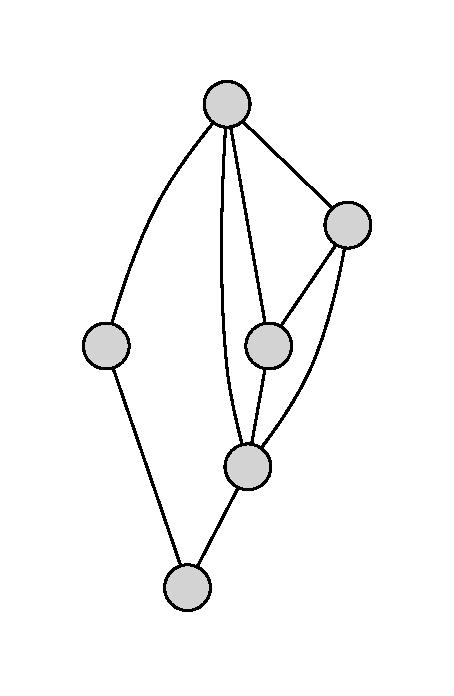
\includegraphics[width=0.5\textwidth]{grafo.pdf}
\caption[Grafo]{Grafo gris.}
\label{imagen:grafo}
\end{figure}

\begin{figure}[ht!]
\centering
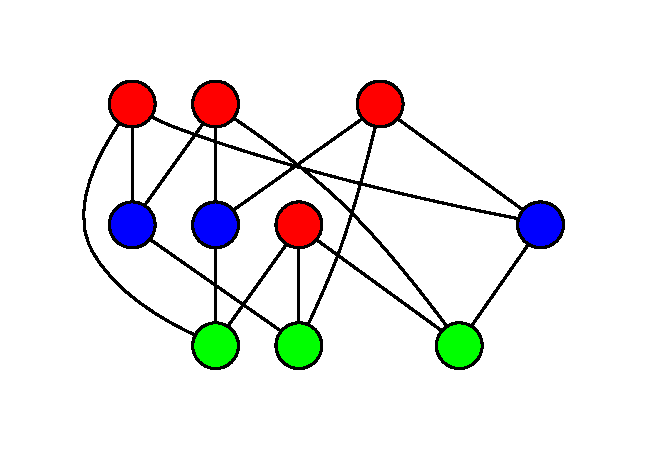
\includegraphics[width=\textwidth]{grafocolor.pdf}
\caption[Grafo coloreado (esto sale en la tabla de contenidos)]{Grafo con color.}
\label{imagen:grafodecolores}
\end{figure}

\chapter{@nombreApendice}
\label{apendiceB}
\lhead{Apéndice B. \emph{@nombreApendice}}

\Blindtext

\addtocontents{toc}{\vspace{2em}}

\backmatter

\end{document}
